\DeclareGraphicsExtensions{.pdf,.jpg,.png}
%--------------- Chapter 3: GRDE ---------------%


\chapter{GREY RELATIONAL BASED KEYPOINTS SELECTION}\label{Ch3:GKS}
\graphicspath{{Chapter3/Chapter3Figs/}{Chapter3/Chapter3Figs/}}

\section{Introduction}\label{ch3:sec:introduction}

Histopathological image classification has grown spaciously and essential for disease analysis. To automatically discriminate benign and malignant images, various classification and feature detection methods are presented in the literature \cite{saraswat2013}. Three types of features can be extracted from the images, namely hand-crafted features, mid-level features, and learned or high-level features. The hand-crafted features, also coined as local features, can be extracted using various popular feature extraction methods, like  LBP (local binary pattern), SIFT, histogram of oriented gradient (HOG) \cite{dalal2005histograms}, and SURF. These methods extract the local visual features from the images. 


In the BOF method, features are extracted from images which are clustered using K-means to generate visual words. The occurrences of visual words in an image can be represented by the histogram which is used to train the classifier. However, this standard method of classification has following demerits \cite{zheng2017}:
\begin{enumerate}
\item All the extracted keypoints are not relevant for the classification and may lead to computationally inefficient image representation.

\item For clustering, K-means is used which has its disadvantages like variance dependency, non-robust, and non-scalable.
\end{enumerate}

To overcome the above mentioned demerits, various methods have been proposed for the selection of relevant keypoints  \cite{brighton2002} \cite{Dorko2003}. Dorko and Schmid \cite{Dorko2003} enhanced the classification performance by applying the SVM on various groups of descriptors to select the most relevant groups. The descriptor vector is divided into groups by the Gaussian mixture model (GMM). Moreover, there are the three best known instance selection algorithms known as IB3 (instance based selection) \cite{aha1991}, DROP3 (reduction techniques for instance-based learning) \cite{wilson2000}, and ICF (iterative case filtering) \cite{brighton2002} with the computational cost of $O(n^2\log_2 n)$, $O(n^3)$, and $O(n^2)$ respectively. Here $n$ denotes the instances. Hence, IB3 is an efficient instance selection algorithm which is further used as a keypoints selection method \cite{lin2016}. However, these methods do not perform well on high dimensional image datasets such as histopathological image datasets. Recently, Lin et al. \cite{lin2016} proposed two iteration keypoints selection methods to improve the bag-of-features but these methods also work on Euclidean distance as similarity measures. On the other hand, histopathological images are very complex having a huge number of keypoints for a single image and there is no method available in the literature for keypoints selection of histopathological images. However, the methods proposed by Lin et. al \cite{lin2016} shows good performance on Caltech image datasets which are less complex as compared to histopathological images and the same method fails to improve the performance to classify the histopathological images. Therefore, an efficient keypoints selection technique based on the grey relational analysis (GRA) is introduced in this chapter which selects comparatively more relevant keypoints. Further, the modified GRA based BOF method is used to classify the histopathological images. The next section presents the BOF approach for histopathological image classification (HIC) followed by the new grey relational analysis based BOF method.

\section{Bag-of-Features Method} \label{ch3:sec:Bag-of-Features Method}

The BOF method is one of the convenient mechanisms for histopathological image classification. It generally consists of five phases as shown in Figure \ref{ch3:fig:BOF_model}:  (i) Setup the image data-store in which  images are organized into predefined categories and partitioned into training and validation subsets, (ii) Extract the texture features or keypoints using feature extraction method, (iii) Cluster the keypoints to generate the visual words, (iv) Encode each image as the histogram of visual words, and (v) Train the classifier using these histograms and corresponding image labels. Finally, the images from the validation set are fed to the trained classifier without a label to predict their labels. Mathematically, the BOF method can be described  as follows:

\begin{figure}
\centering
     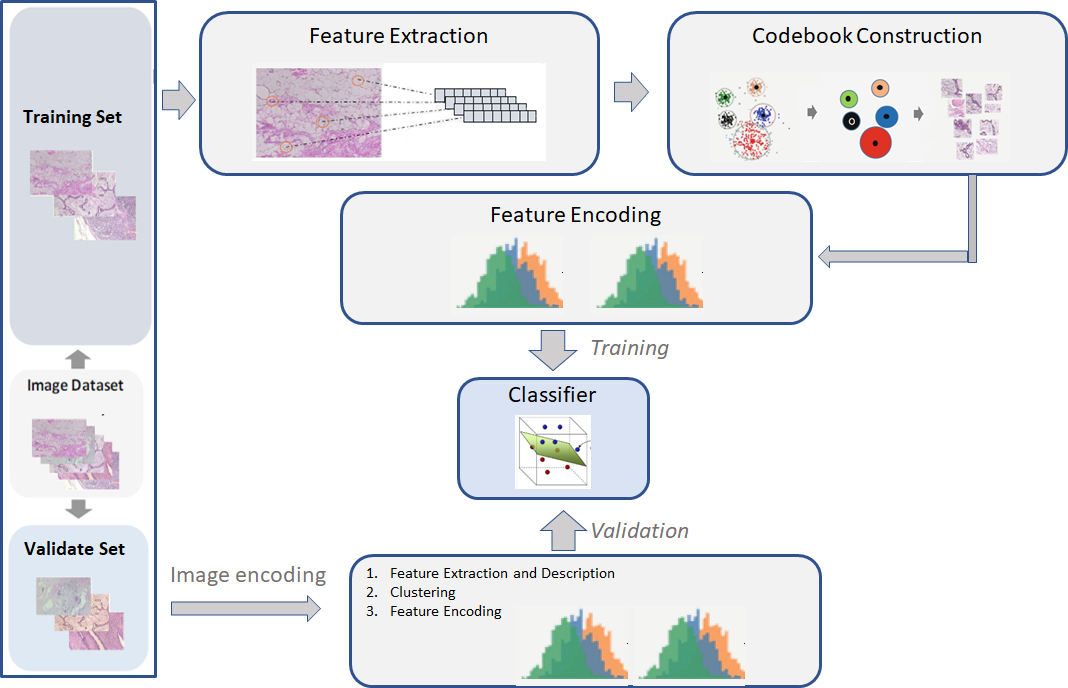
\includegraphics[width=1.0\textwidth]{BOVW2}
   \caption[The architecture of the BOF method]{\fontsize{10}{12}\selectfont The architecture of the BOF method}
 \label{ch3:fig:BOF_model}
\end{figure} 

\begin{enumerate}
  \item  \textbf{Dataset partition:} Let $C= \{c_1, c_2, \dots, c_i, \dots c_n\}$ is a set of $n$ classes. Each class $c_i$ is associated with a set of images. The image dataset is divided into two parts. One is a training set on which the classifier is trained and the other is a validation set, which is used to validate the trained classifier. The training set of $N$ images is prepared by randomly selecting $M_i$ images from each class $c_i$ which is also given by  Eq. (\ref{eq:Ttotal}). The remaining images of the classes are considered as a part of validation set.
\begin{equation} \label{eq:Ttotal}
N= \sum_{i=1}^n M_i
\end{equation}

  \item \textbf{Feature extraction:} Extract the keypoints from all $N$ images of training set using a feature extraction method like, SURF \cite{bay2008}, FREAK \cite{alahi2012}, SIFT \cite{lowe2004}, and HOG \cite{albiol2008}. Let $X$ is a set of keypoints, defined as Eq. (\ref{eq:Xaa}). 

\begin{equation}\label{eq:Xaa}
X= [F_1, F_2, \dots, F_N]^T
\end{equation} 
 where, $F_i$ is a matrix of  $P$ keypoints for the $i^{th}$ image, defined over $d$-dimensional space and is given by Eq (\ref{eq:Xaa1}). 

\begin{equation}\label{eq:Xaa1}
F_i=     \left\{\begin{array}{c}
f_{11} \  \ f_{12}\  \  f_{13} \ \  \dots \ \ f_{1d}\\ 
f_{21} \ \ f_{22} \ \ f_{23}  \ \ \dots  \ \ f_{2d}\\
\dots \ \ \dots \ \ \dots \ \ \dots \ \ \dots \\
f_{P1} \ \ f_{P2} \ \ f_{P3}  \ \   \dots \ \  f_{Pd}
\end{array}\right\}
\end{equation} 

Figure \ref{ch3:fig:kp} shows representative keypoints detected by one of the feature extraction method i.e., SURF from two images, randomly taken from the two considered histopathological image datasets. Each image is first converted to grayscale then SURF detector is used to find the predefined number of keypoints from these images. In the figure, only $40$ strong keypoints are depicted for simplicity and visualization.

\begin{figure}
\centering
    \subfigure[]{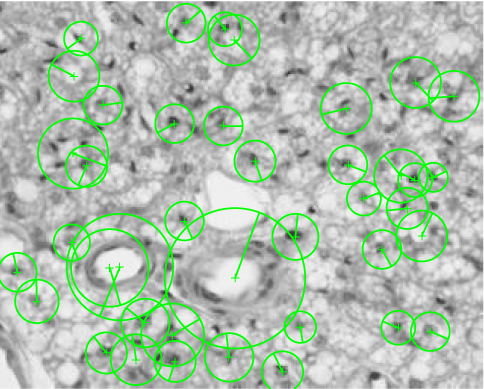
\includegraphics[scale=1.3]{Connective}}~~~~~
    \subfigure[]{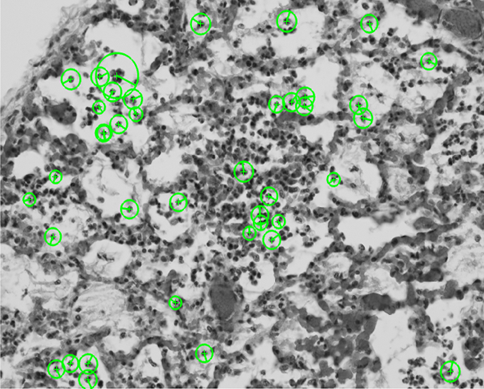
\includegraphics[scale=1.3]{lung}} 
 \caption[The keypoints detected by SURF in connective tissue and inflamed lung histopathological images]{ \fontsize{10}{12}\selectfont The keypoints detected by SURF in (a) connective tissue image and (b) inflamed lung tissue images}
\label{ch3:fig:kp}
\end{figure}

\item\textbf{Codebook construction:} Create visual words by iteratively grouping the extracted descriptor vector $X$ into $n$-mutually exclusive clusters. Each cluster can have any number of keypoints based on the similitude of the intensity values of pixels in an image with the extracted keypoints. For the same, $K$-means algorithm is used and the returned cluster centers are represented as visual words.  

\item \textbf{Encoding:} Encode each image into a histogram ($H_j=\{H_{j1}, H_{j2}, \dots, H_{jn}\}\ for\  j=1, 2, \dots, N$), representing the visual word occurrences in each image which is given by Eq. (\ref{eq:jk}). 

\begin{equation} \label{eq:jk}
H_{jk}= \sum_{i=1}^P \mu_{ik}(j)  \ \ where \ \ k=1, 2, \dots, n 
\end{equation}

\begin{equation} \label{eq:pk}
\mu_{ik}= \begin{cases}1 & if \ \ \parallel v_k - f_i \parallel \leq \parallel v_s - f_i \parallel \ \ for \ \ s=1,2,\dots, n, \\0 & otherwise\end{cases}
\end{equation}

where, $P$ represents the number of keypoints  and $\mu_{ik}(j)$ is $1$ when any visual word ($v_k$) is close to any keypoint $f_i$ in the image. This method is also known as vector quantization.

\item \textbf{Classification:} Each histogram ($H_j$) along with its annotation is used to train the classifier for the image classification task.  Once the classifier is trained, it is tested to predict the label of images provided in the validation set. Each validation image is represented as the histogram as discussed above and fed to the classifier without a label. Based on the returned label by the classifier, its accuracy is measured.
\end{enumerate}

In the feature extraction phase of the BOF method, a feature detection and representation method is used to find the keypoints in the images. These keypoints are then represented as the descriptor vectors which are further used for codebook construction. Out of many feature extraction methods, SURF is the fastest method because it uses box filters for the convolution of images and converts each image as the integral image. It extracts the texture features from the images \cite{bay2008}. Moreover, SURF is a resolution invariant feature detector, hence images of different resolutions do not have any impact on the classification performance. This property of SURF helps to analyze the histopathological images, having different resolutions (e.g., 10x, 20x, 40x) \cite{xu2013}. The interest points in the images are detected using the Hessian matrix approximation. SURF also shows good performance over other alternatives like SIFT  \cite{juan2009}. Therefore, this work uses SURF to extract a set of keypoints ($X$) from $N$ training images.
        
Generally, SURF extracts a large number of keypoints due to the complex texture of histopathological images. This reduces the efficiency of visual vocabulary generation \cite{lin2016}. Furthermore, all of the detected keypoints are not necessary for image classification and annotation \cite{lin2016}. Hence, an efficient keypoints selection method is required for the acquisition of relevant keypoints that can improve the speed and efficiency of the BOF method.  Some of the popular keypoints selection techniques are IB3 \cite{aha1991} and iterative keypoints selection (IKS1, IKS2) \cite{lin2016}. IB3 is an efficient instance selection method with high space complexity while IKS1 and IKS2 are the keypoints selection methods that are used to find representative keypoints from the images. IKS1 and IKS2 are differed by their initial representative keypoints selection methods. In IKS1, representative keypoints are selected randomly while in IKS2, cluster centers are considered as representative keypoints. The remaining keypoints are eliminated based on their Euclidean distances from the selected representative keypoints. However, Euclidean distance similarity measure is computationally expensive for high dimensional data. Chang et al. \cite{chang2005} has shown that computational cost of Grey relational analysis (GRA) \cite{julong1989} based similarity measure is better than the Euclidean distance based similarity.  Therefore, in this work, a new GRA based keypoints selection (GKS) method is introduced to reduce the number of keypoints before feeding them into the next phase of the BOF method i.e., codebook construction. The modified flow of the BOF method is depicted in Figure \ref{ch3:fig:mbof}. The next subsection provides a detailed description of the new grey relation analysis based keypoint selection method. 

\begin{figure}[t]
            \centering
            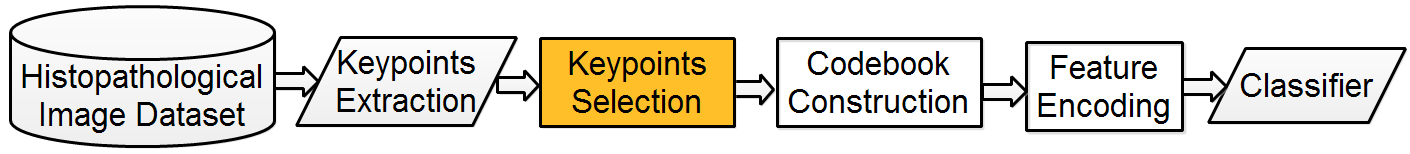
\includegraphics[width=1.0\textwidth]{BOF}
            \caption[Flow chart of the enhanced BOF method]{\fontsize{10}{12}\selectfont Flow chart of the enhanced BOF method}\label{ch3:fig:mbof}
\end{figure}



\section{Grey Relational Analysis based Keypoints Selection} \label{ch3:sec:Grey Relational Analysis based Keypoints Selection}

The GKS method uses the concept of grey relational analysis for finding the similarity between the keypoints. GRA \cite{julong1989} is a part of Grey system theory which is used to examine the similarity between data tuples based on geometrical mathematics \cite{sallehuddin2008}. It conforms to four basic principles in the dataset, i.e., proximity, normality, symmetry, and entirety \cite{wang2001}. In GRA, the similarity between a reference tuple and the remaining tuples for a given data is computed by Grey relational grades (GRGs) whose value lies between $0$ and $1$. For any data tuple, if GRG is close to $1$, then it is highly similar to the reference tuple while the dissimilarity will be signified if GRG value is close to $0$ \cite{chang2005}. 

Therefore, the new keypoints selection method uses GRA to eliminate similar keypoints from the feature descriptor, generated by SURF. The new GKS method has the following steps:

\begin{enumerate}
\item Cluster the keypoints into $K$ clusters using approximate K-means  (AKM) algorithm \cite{wang2015}.
\item Make the cluster centers as the member of selected keypoints set and also consider them as reference points for the computation of GRGs for the remaining keypoints.
\item Compute the GRG values between the reference point and the keypoints lying within the corresponding cluster.  The mathematical formulation of GRG computation is described below.

Let $X_o={X_{r1}, X_{r2}, \dots, X_{ri}, \dots, X_{rn}}$ be a set of $n$ reference points. The elements in $X_o$ are of the form $X_{ri}=\langle X_{ri}(1), X_{ri}(2), \dots, X_{ri}(u) \rangle$, where $u$ corresponds to the dimension of the extracted keypoint. Similarly, let $X_c={X_{c1}, X_{c2}, \dots, X_{cm}}$ be a set of $m=P-n$ remaining keypoints considered as comparative keypoints where, each element in $X_c$ can be denoted as $X_{cj}=\langle X_{cj}(1), X_{cj}(2), \dots, X_{cj}(u) \rangle$.  The GRG value of each keypoint in $X_c$ is given by Eq. (\ref{eq:grg}) \cite{chang2005}.
\begin{equation} \label{eq:grg}
GRG (X_{oi}, X_{cj})= \sum_{t=1}^u[\alpha_i(t) \cdot GRC(X_{oi}(t), X_{cj}(t))]
\end{equation}
where, GRC is the grey relational coefficients and  $\alpha_i(t) = \frac{1}{u} $ is the weighting factor of GRC. The GRC value, between $i^{th}$ keypoint of $X_o$ and $j^{th}$ keypoint of $X_c$ at $u^{th}$ datum, belonging to the $i^{th}$ cluster only is given by Eq. (\ref{eq:grc}) \cite{chang2005}.

\begin{equation} \label{eq:grc}
GRC(X_{oi}(u), X_{cj}(u))=\frac{ \min \limits_{ij}  \triangle_{ij}(u) + \xi \max \limits_{ij} \triangle_{ij}(u) }{\triangle_{ij}(u)+\xi \max\limits_{ij} \triangle_{ij}(u)}, 
\end{equation}
where,  $\xi \in (0,1]$ is a random number to control the constancy between  $\max\limits_{ij} \triangle_{ij}(u)$ and $ \min \limits_{ij}  \triangle_{ij}(u)$.  $ \triangle_{ij}(u)$ is computed by $\mid X_{oi}(u) - X_{cj}(u) \mid$ for $i=1, 2, \dots, n$, $j=1, 2, \dots, c$.
\item In every cluster, the above computation is performed to find the highly similar points with cluster center and eliminate $s\%$ of the keypoints from each cluster whose GRG values are higher, in their corresponding cluster. Here, $s$ is termed as shrinking threshold. 
\item Repeat the steps 1 to 4 till the remaining keypoints are greater than $K$ and add  the last set (having $K$ points only) of cluster centers to the selected keypoints set.

\item Use the selected keypoints set as input to the next phase of BOF i.e., codebook construction.
\end{enumerate}

After finding the optimum keypoints from the new GKS method, the codebook construction phase of BOF (as described in Section \ref{ch3:sec:Bag-of-Features Method}) is performed which uses K-means clustering to generate various visual words. Further, the frequencies of each visual word in the images are represented by histograms. These histograms along with the corresponding image labels are given to  SVM for training which is further used for image classification.

\section{Experimental Results} \label{ch3:sec:expr}

The performance of the GKS method is analyzed in three phases on two histopathological image datasets. First, it is compared with the state-of-the-art keypoints selection methods in Section \ref{subsec:1}. Second, the results of the GKS based BOF method for classifying histopathological images are presented in Section \ref{subsec:2}. In the third phase, the performance of the new classification method has been analyzed against three state-of-the-art classification methods in Section \ref{ch3:subsec:3}. 

\subsection{Datasets}\label{ch3:subsec:dataset}
Two standard histopathological image datasets are considered for the classification task, namely ADL histopathological image dataset and Blue histology image dataset which are described below.

\begin{itemize}
\item \emph{ADL histopathological image dataset \cite{srinivas2014}}: This dataset contains images of three bovine organs, namely Kidney, Lung, and Spleen. These images are further divided into two subcategories: healthy and inflammatory. Sample images are depicted in Figure \ref{ch3:fig:ADLdataset} Each image is stained with hematoxylin and eosin (H\&E) dye. The inflammatory tissue images, having some specific white blood cells, are used to identify the reason and duration of the infectious diseases. The presence of eosinophil cells in tissue indicates the inflammations such as parasites, allergic infections, or bacteria.  There are two types of infections in the organs, acute and chronic, which can be recognized by the neutrophils cells and lymphocytes cells respectively in the tissues. From Figure \ref{ch3:fig:ADLdataset}, it can be observed that in the inflamed lung, the alveoli are not clear as healthy lungs have, but it is filled with bluish-purple inflammatory cells. Similarly, inflammation in other organs is also indicated by dark blue nuclei. This dataset contains $120$ images per organ. This dataset is taken from Animal Diagnostics Lab (ADL), Pennsylvania State University.  The ground truth label for each image is assigned by ADL pathologists by performing manual segmentation and detection of healthy and inflammatory tissues. These tissue images have special biological structures with different conditions. The infectious tissue is generally an indication of the transferable disease.  
\begin{figure}[h]
\centering
        \subfigure[Healthy Kidney]{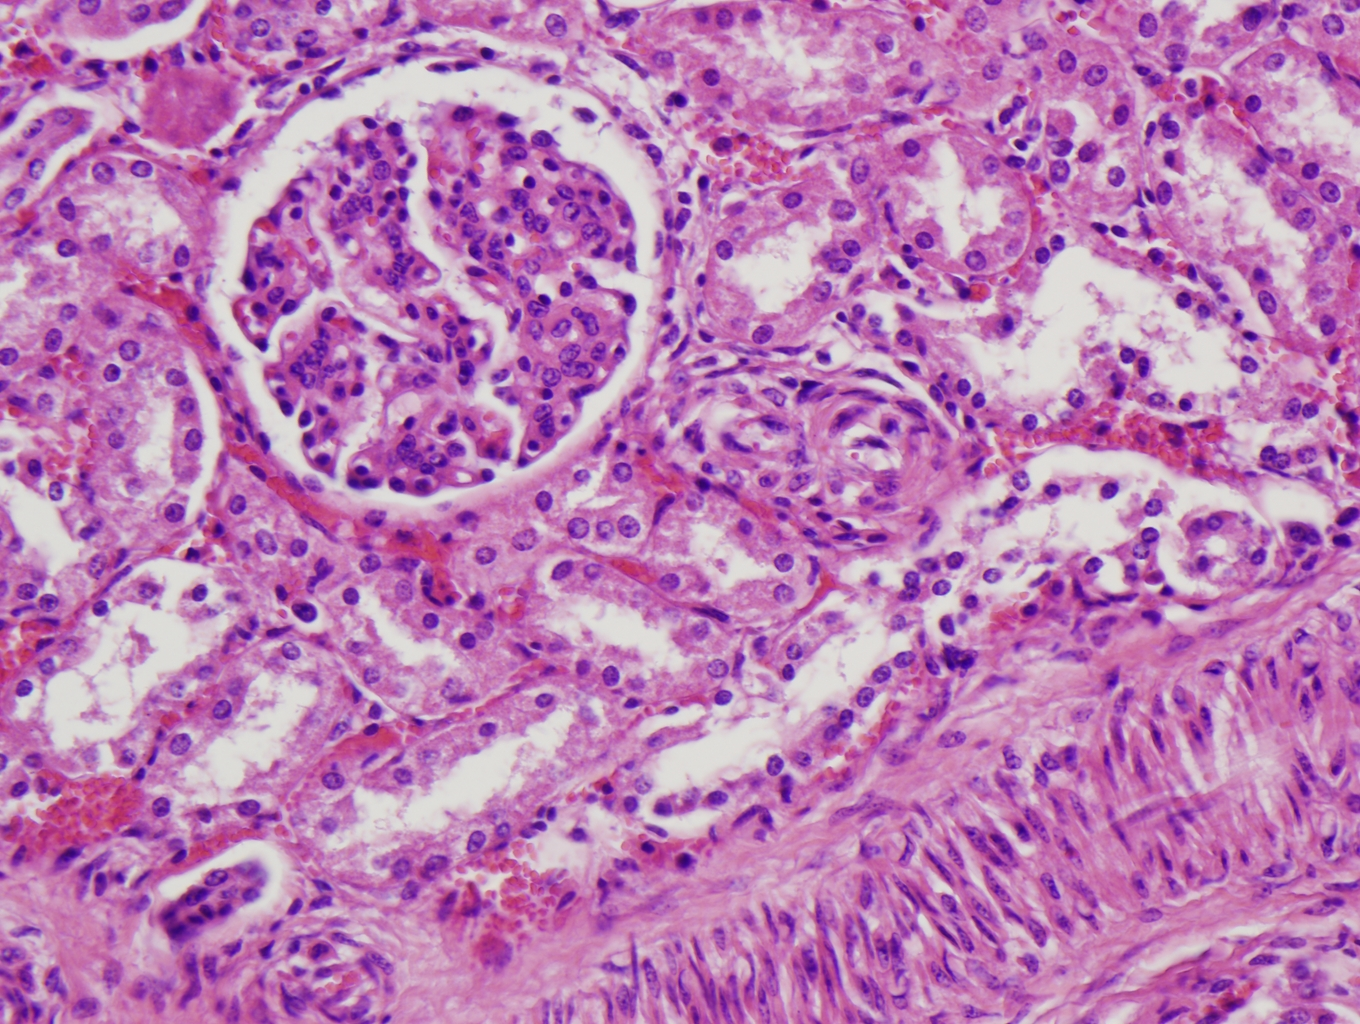
\includegraphics[width=1.2in, height=0.8in]{KN}} \hspace{2mm}
            \subfigure[ Inflamed Kidney]{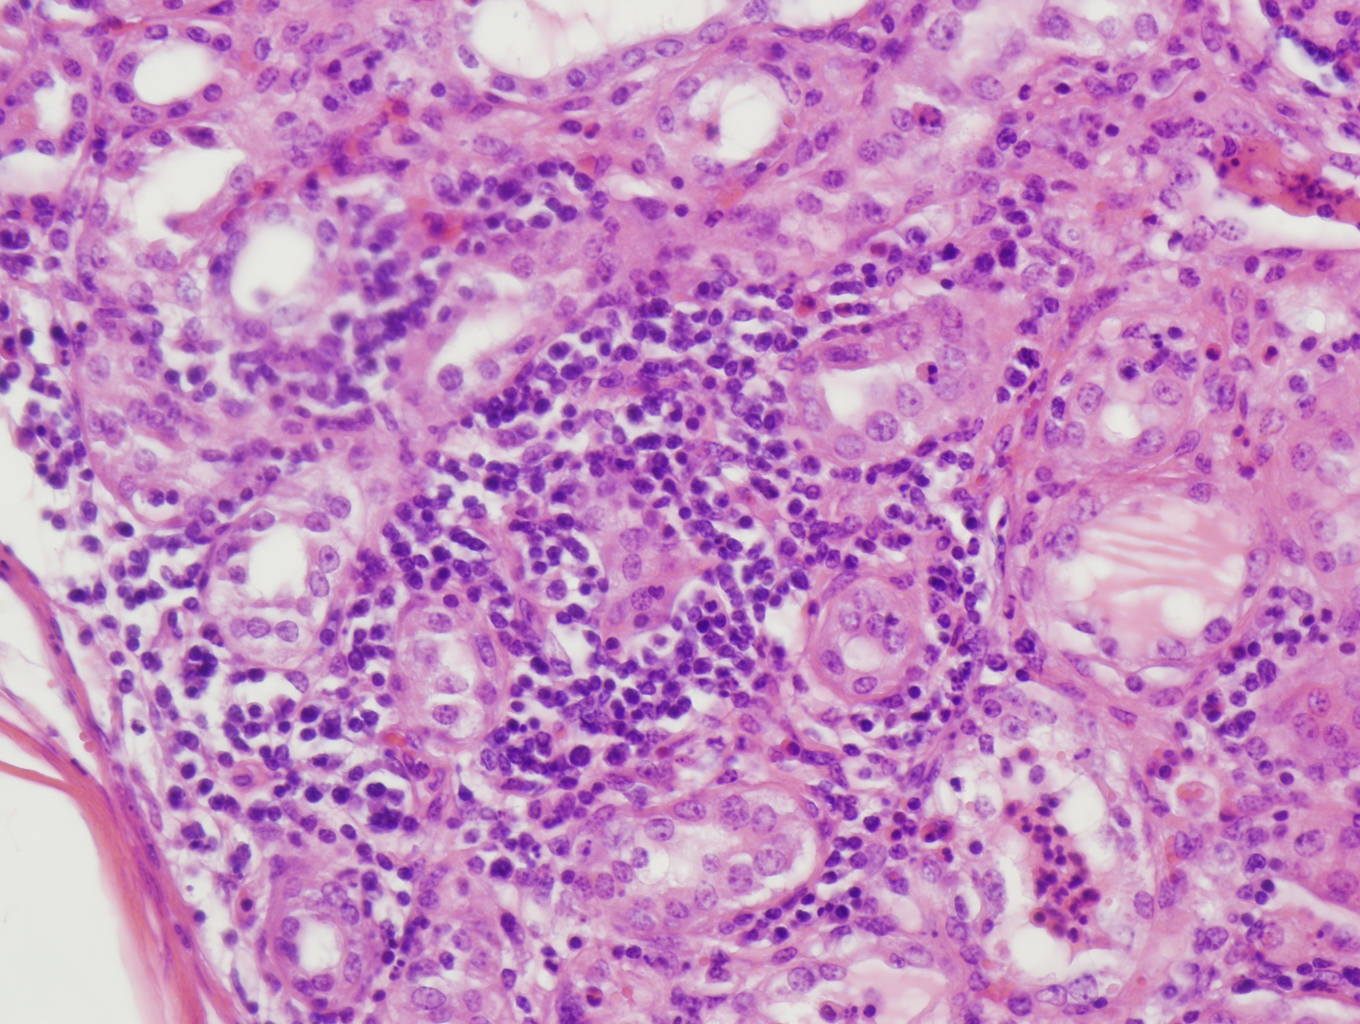
\includegraphics[width=1.2in, height=0.8in]{KI}} \\
        \subfigure[Healthy Spleen]{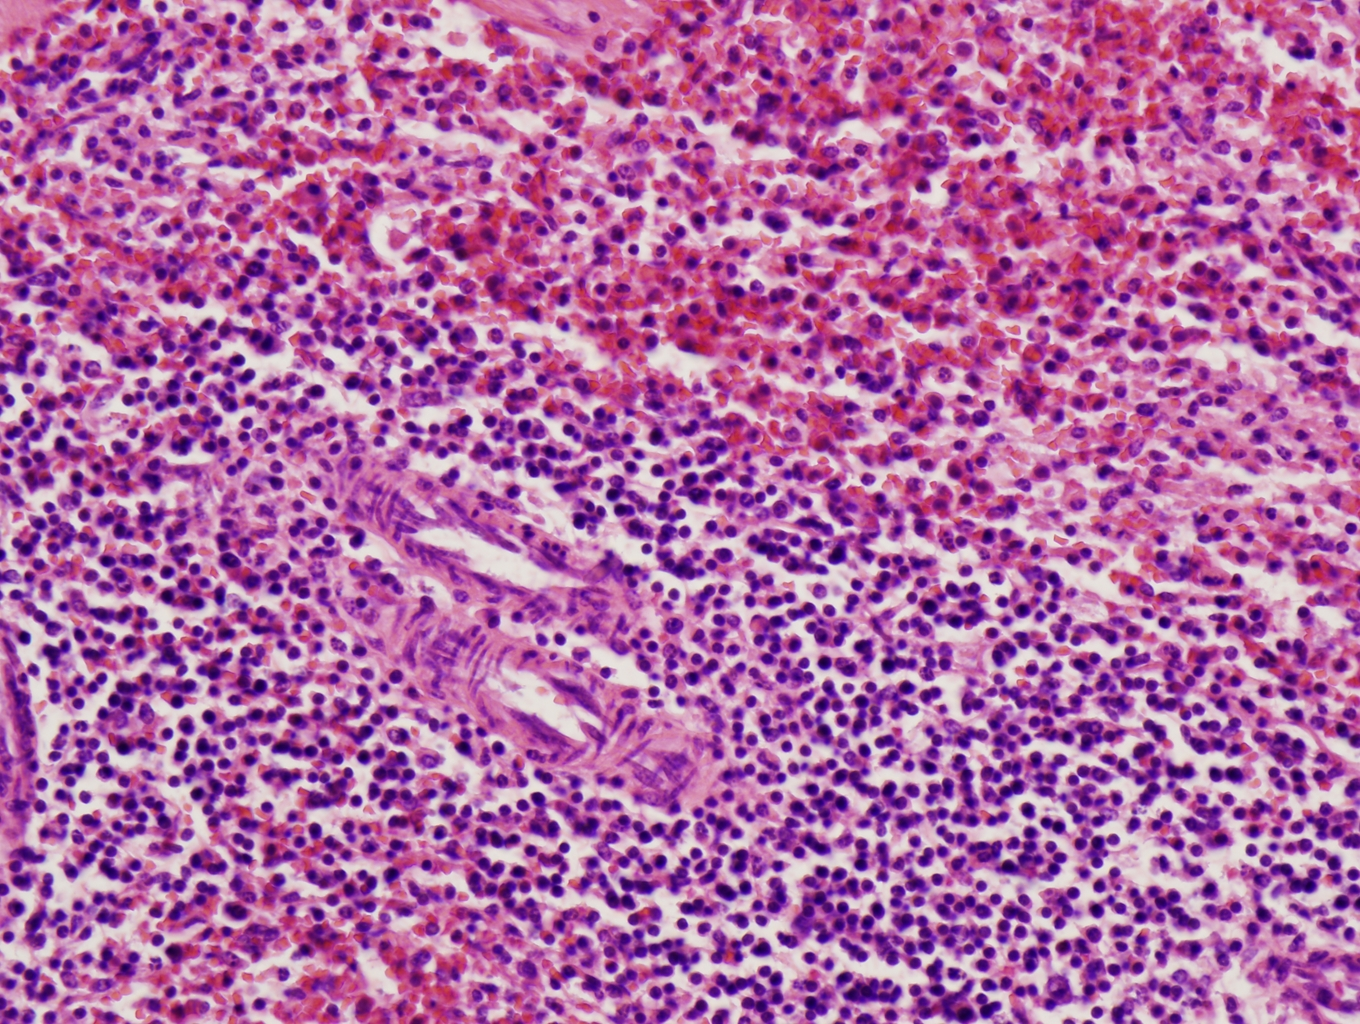
\includegraphics[width=1.2in, height=0.8in]{SN}}\hspace{2mm} 
        \subfigure[Inflamed Spleen]{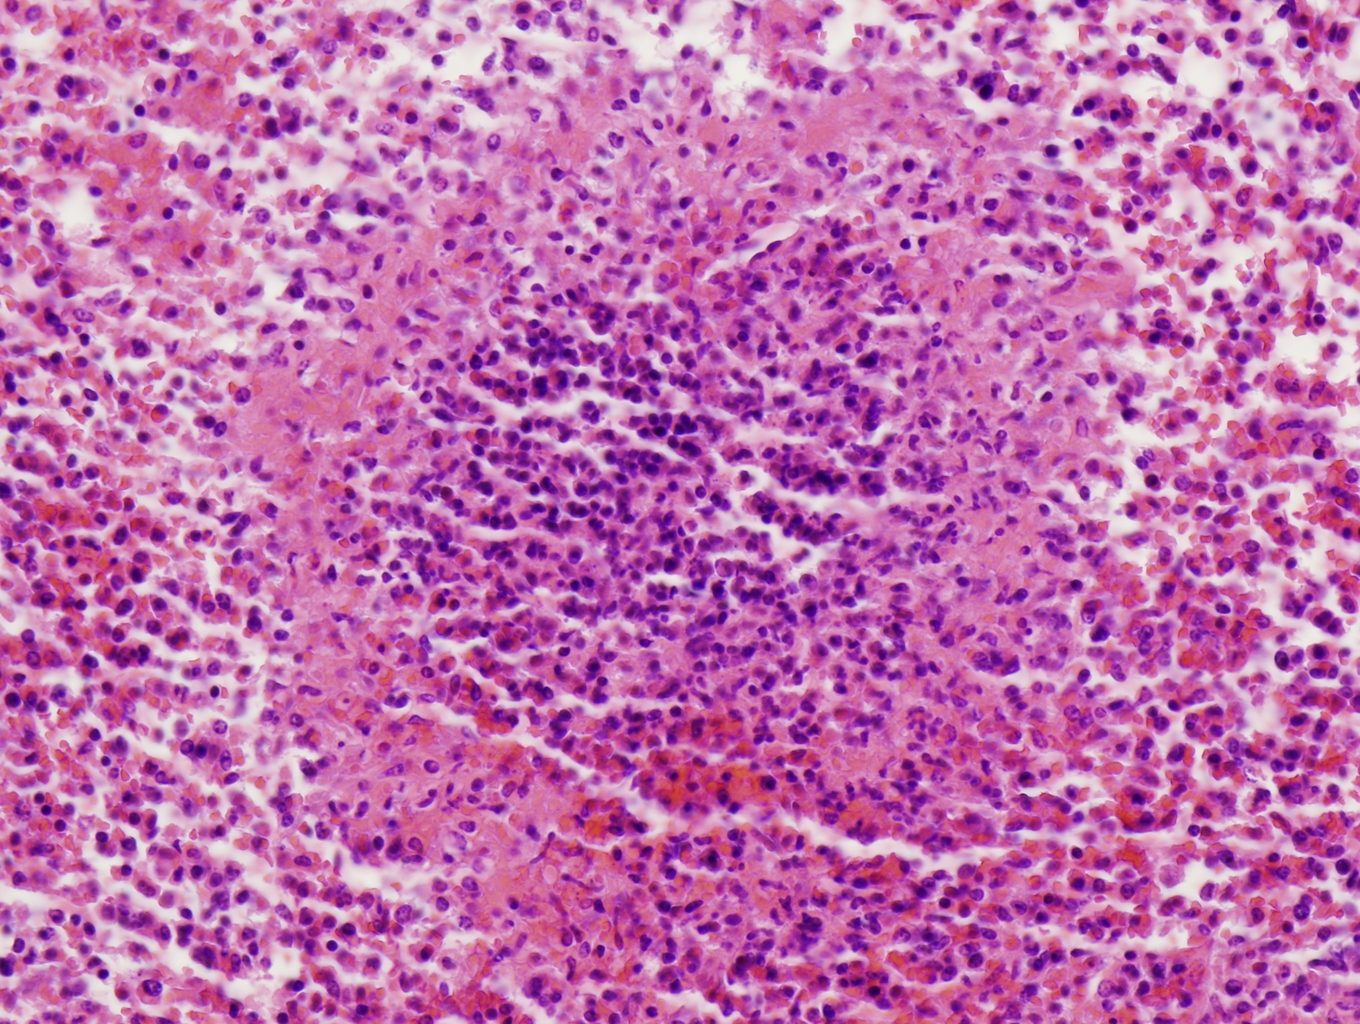
\includegraphics[width=1.2in, height=0.8in]{SI}}\\
        \subfigure[ Healthy Lung]{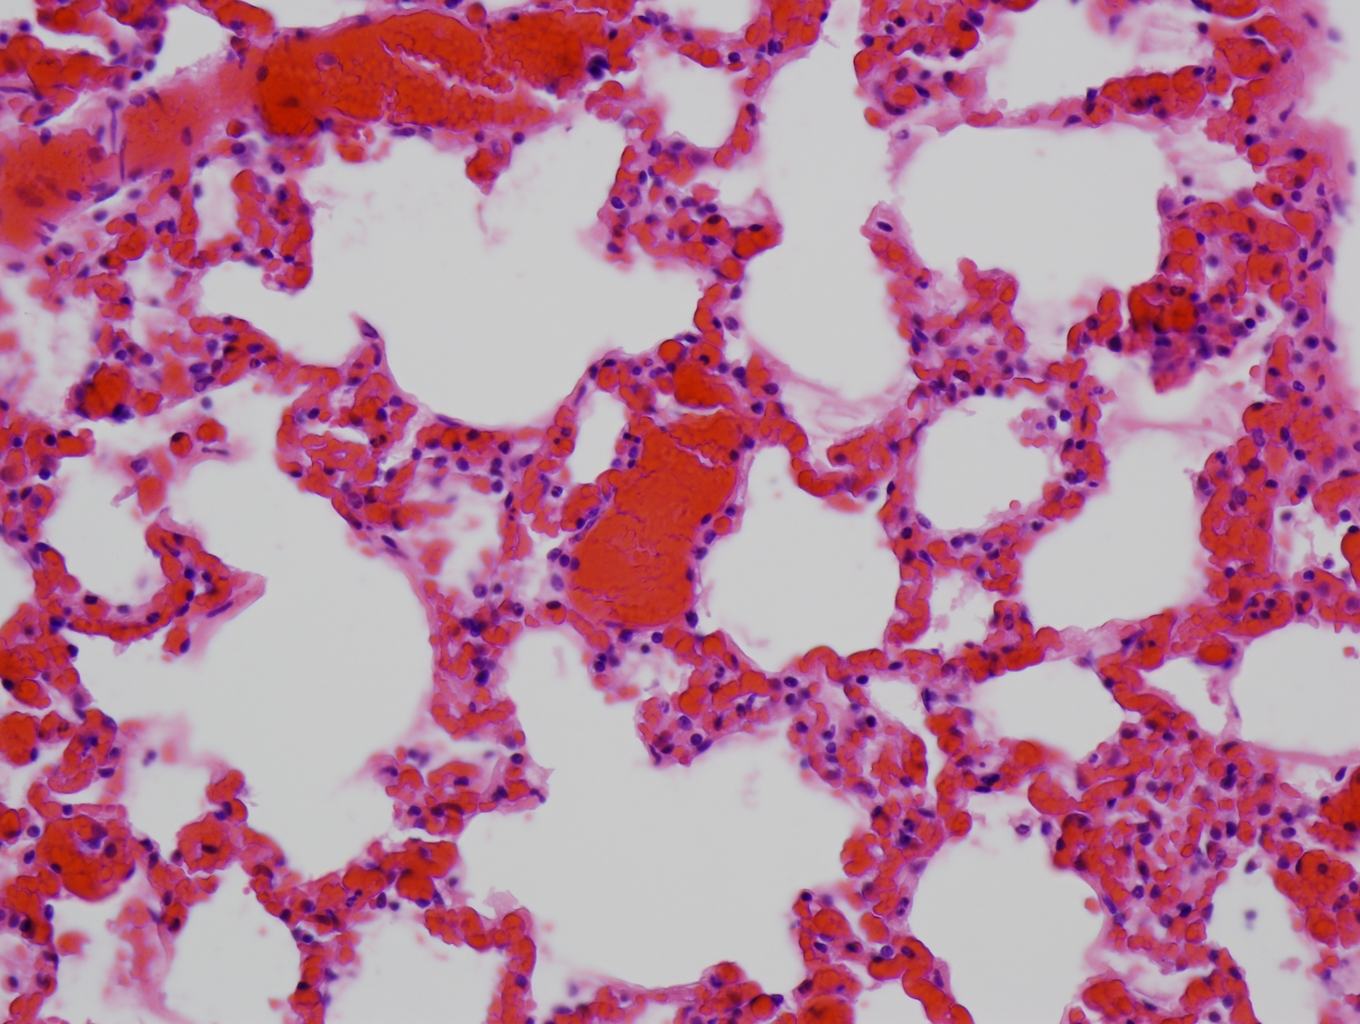
\includegraphics[width=1.2in, height=0.8in]{LN}}\hspace{2mm}
        \subfigure[Inflamed Lung]{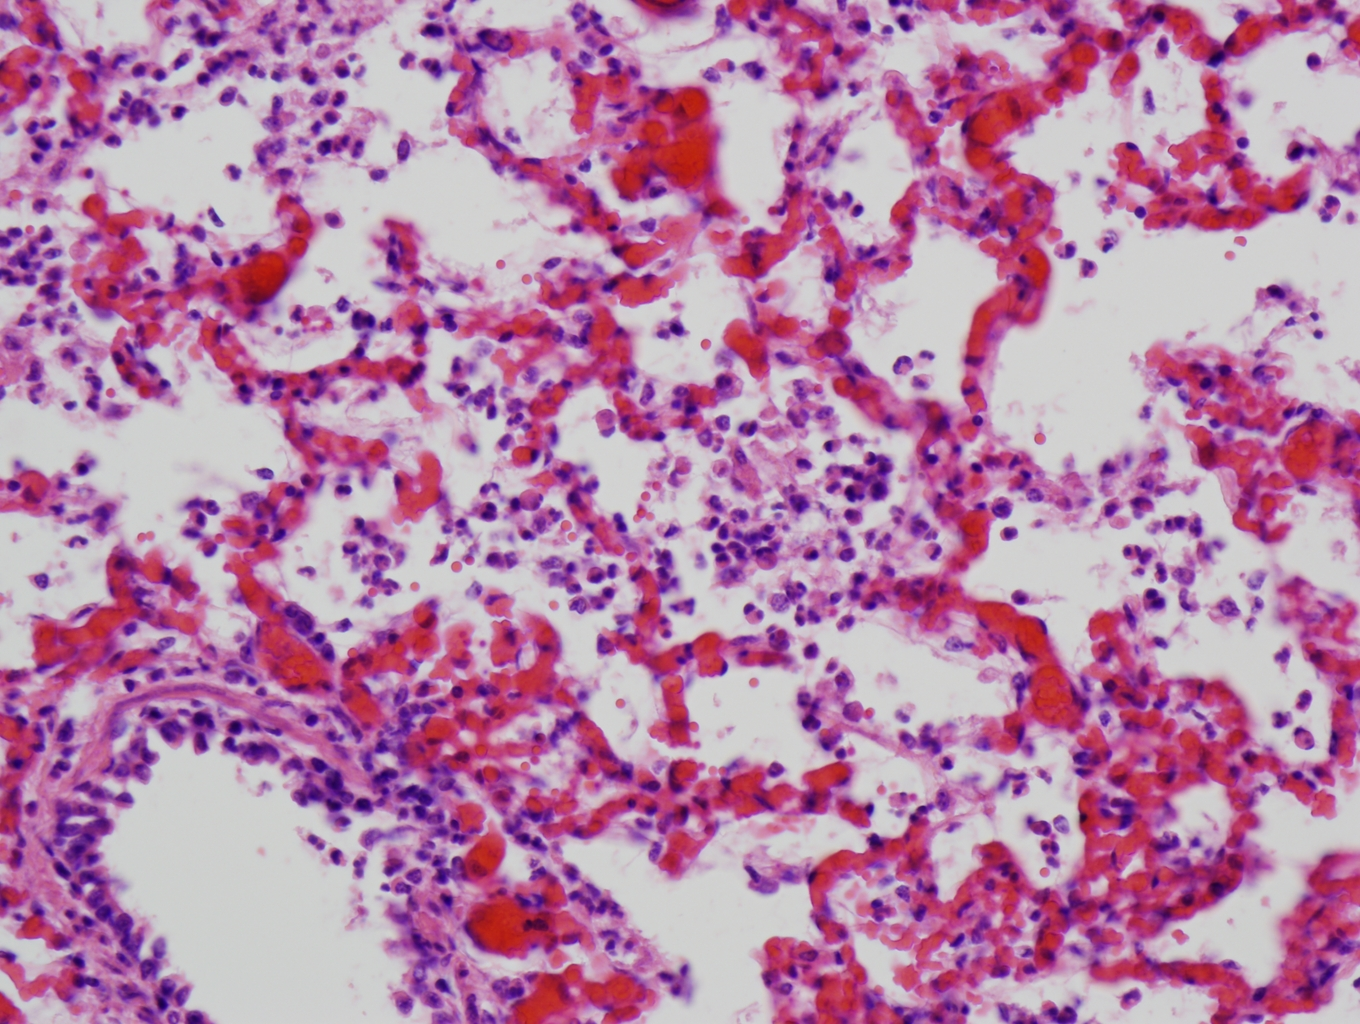
\includegraphics[width=1.2in, height=0.8in]{LI}}
  \caption[Healthy and inflammatory tissues of Kidney, Lung, and Spleen]{\fontsize{10}{12}\selectfont Ground truth labels for healthy and inflammatory tissues of Kidney, Lung, and Spleen \cite{srinivas2014}}
\label{ch3:fig:ADLdataset}
\end{figure}


\item \emph{Blue histology image dataset \cite{BlueHist:online}}: This dataset consists images of four tissues, namely epithelium, connective, muscular, and nervous. Epithelium tissues include those cells that cover the organ surfaces like skin surfaces and digestive tract inner lining. The cells are linked together by the epithelial layer to provide a fence between the organ and the external environment. Epithelium tissues help to protect organs from laceration, fluid loss, and microbe. Connective tissues are gristly tissues made up of an extracellular matrix. These tissues provide shape to organs and bind them in place. Examples of connective tissues include ligament, blood, tendon, and areolar tissues. Muscle tissues are the active contractile tissues of the organ formed by muscle cells. These tissues generate a force that results in movement within internal organs or locomotion. Nervous tissues consist of different nerve cells having an axon, which are responsible for sending an activation signal to the subsequent cell. These tissues are the component of the brain and spinal cord nervous system \cite{eurell2013}.  Figure \ref{ch3:fig:tissue} shows sample images taken from each type of tissue images. Each image category contains 101 tissue images. Moreover, various staining methods are used to provide colors for each category tissue images and the brief description of staining methods along with tissue category is depicted in Table \ref{ch3:tab:tissued}.

\begin{figure}
\centering
        \subfigure[ET]{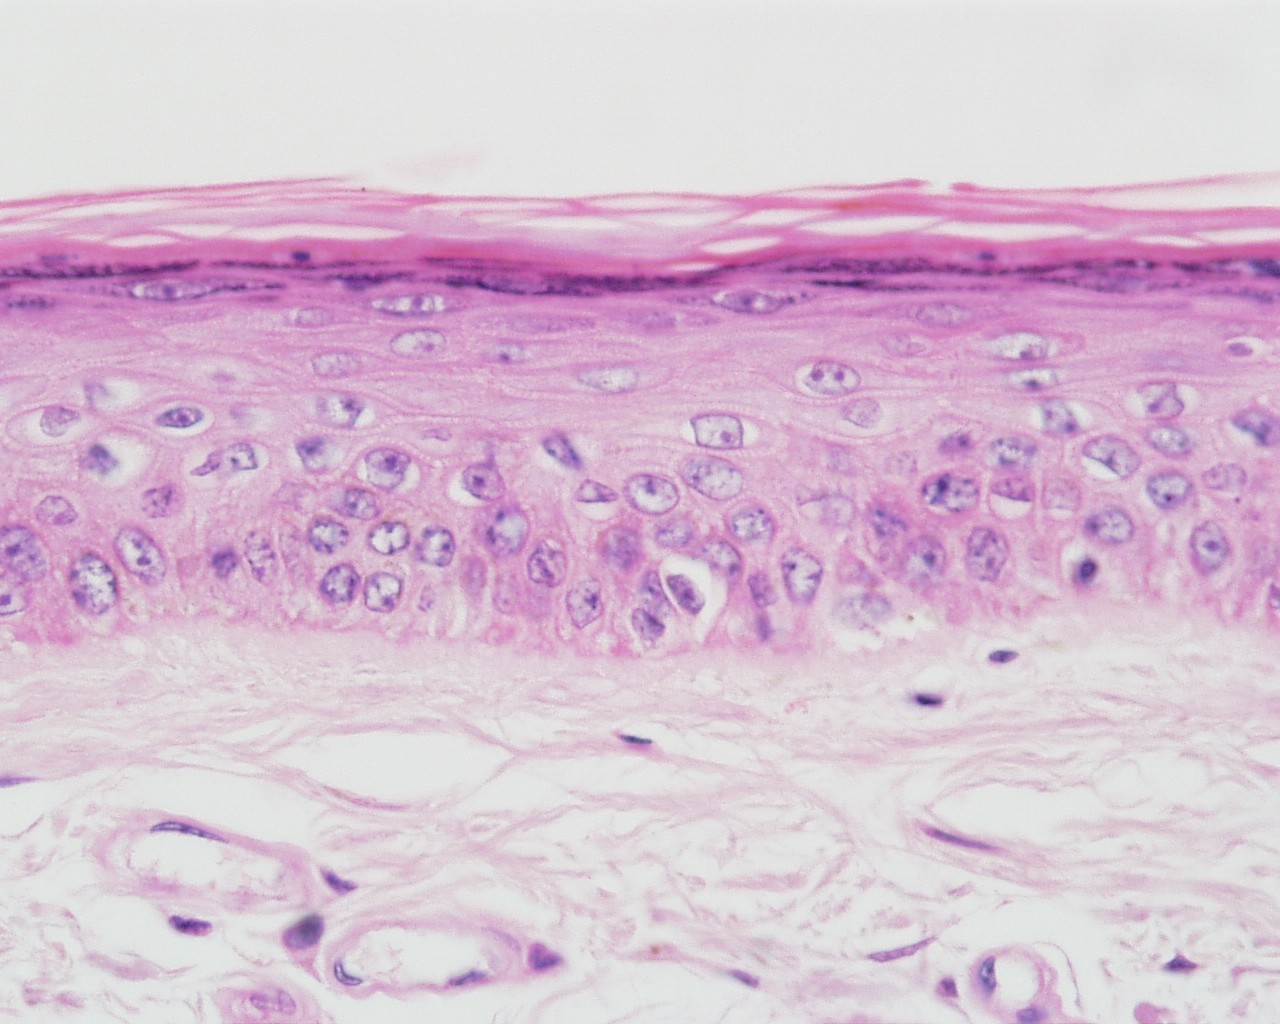
\includegraphics[width=0.22\linewidth]{ET}} \hspace{1mm}
            \subfigure[CT]{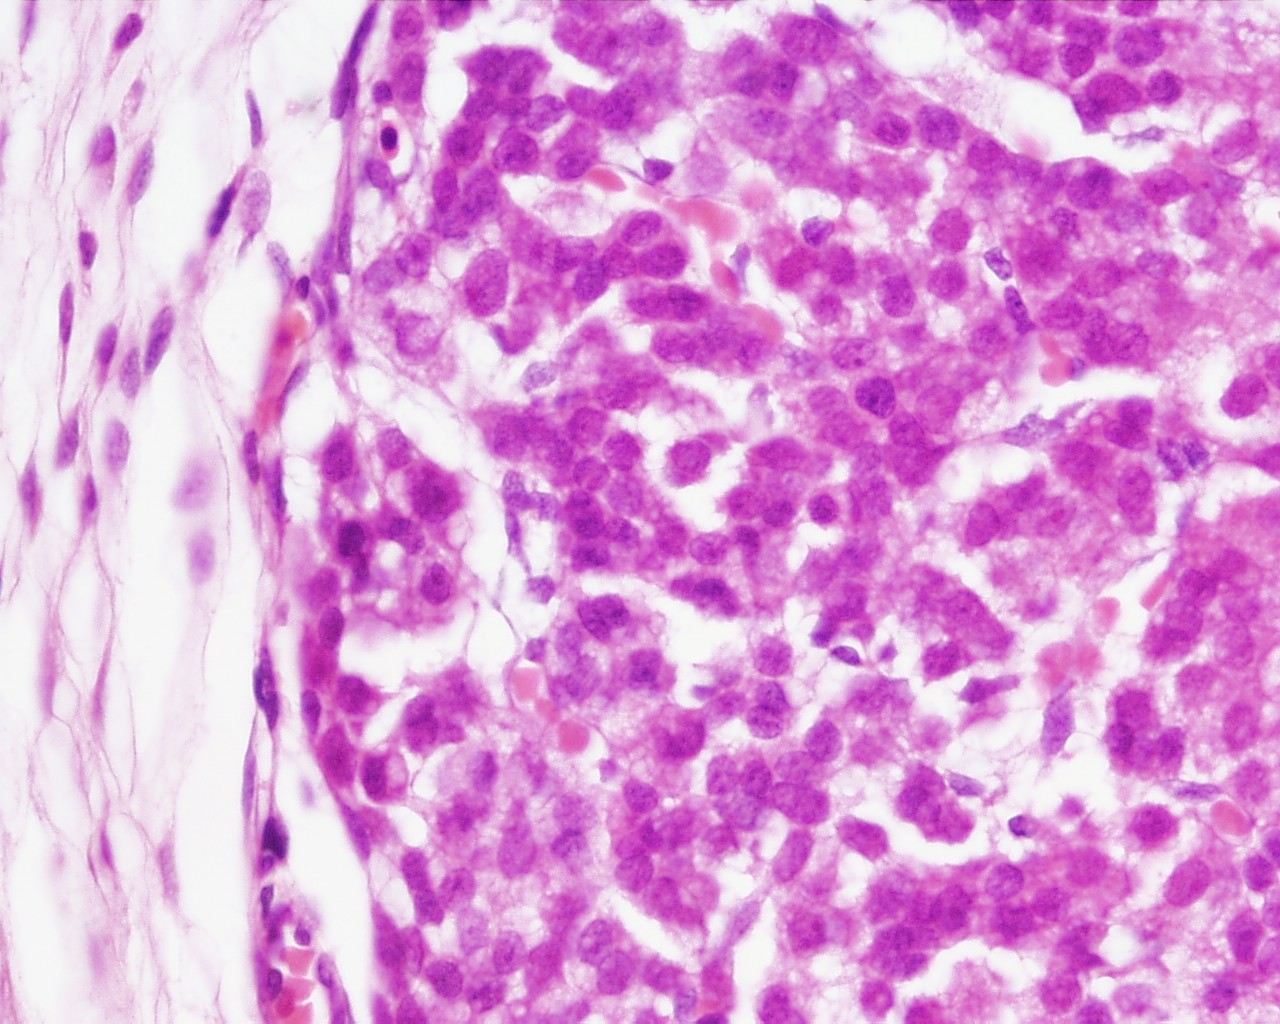
\includegraphics[width=0.22\linewidth]{CT}}\hspace{1 mm}
        \subfigure[MT]{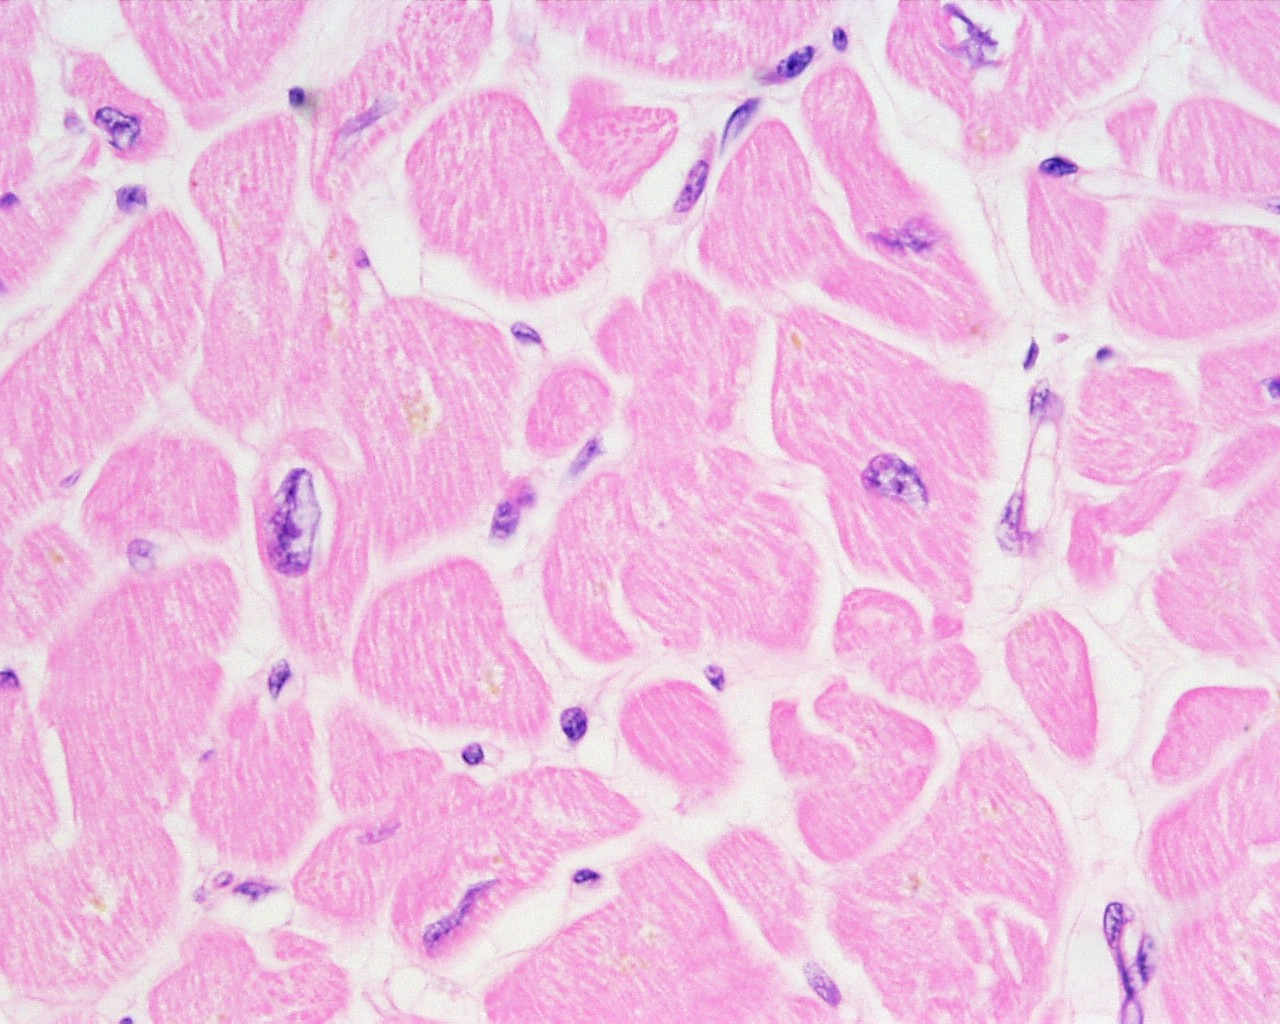
\includegraphics[width=0.22\linewidth]{MT}} \hspace{1mm}
        \subfigure[NT]{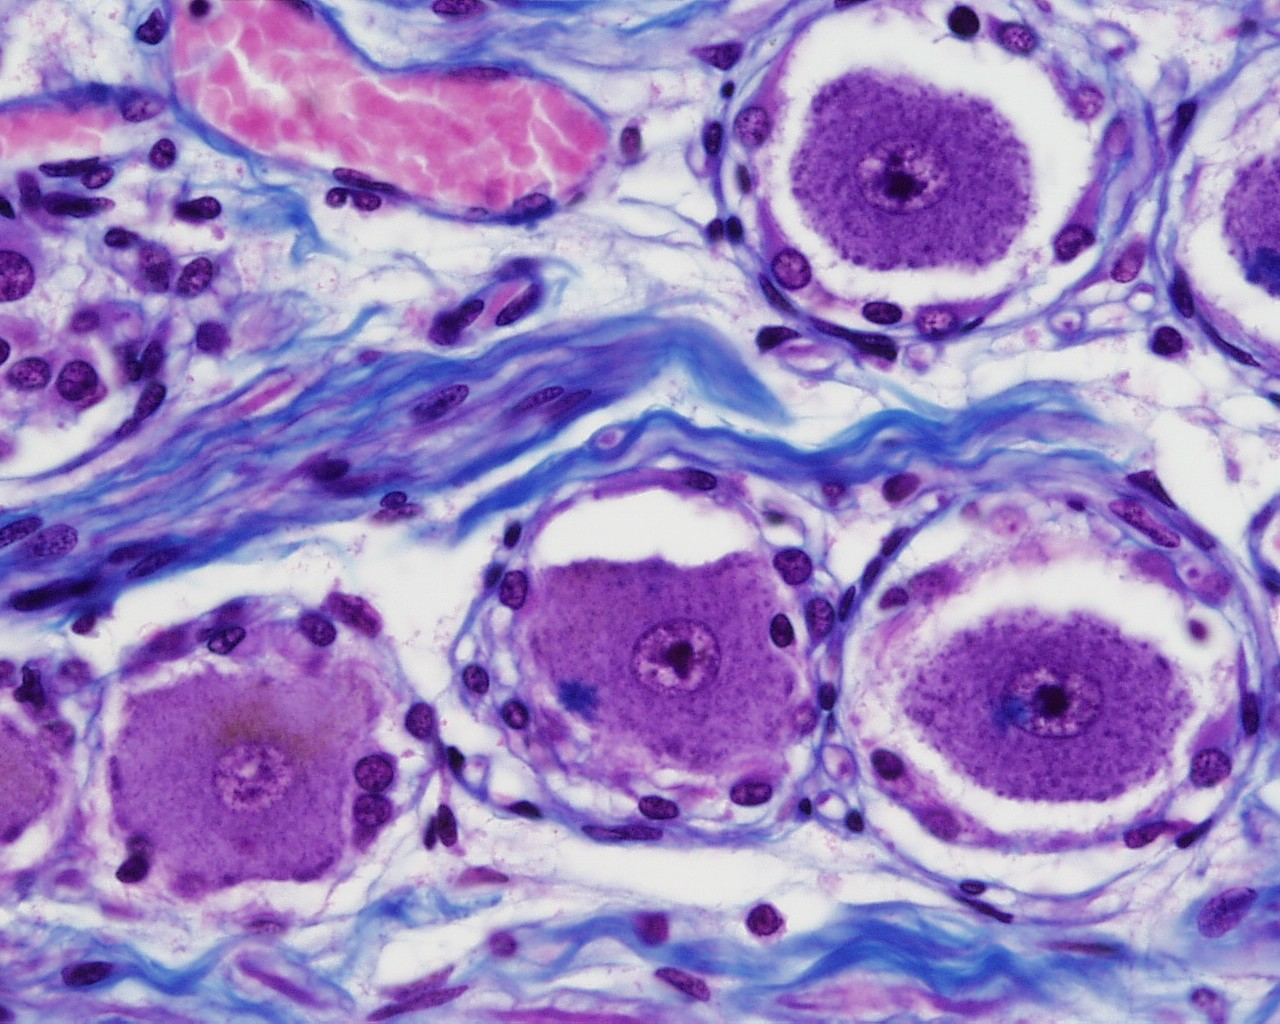
\includegraphics[width=0.22\linewidth]{NT}}
  \caption[Representative animal tissues from blue histology dataset at $40 \times$  magnification level]{\fontsize{10}{12}\selectfont Representative animal tissues from blue histology dataset at $40 \times$  magnification level \cite{BlueHist:online}. Here, CT: Connective Tissue, ET: Epithelial Tissue, MT: Muscle Tissue, and NT: Nervous Tissue.}
\label{ch3:fig:tissue}
\end{figure}

\begin{table}[h]
\caption[The different categories of histology image dataset and their staining methods]{\fontsize{10}{12}\selectfont The various tissue categories of blue histology dataset with  their staining methods}
\label{ch3:tab:tissued}
\centering
\footnotesize
\renewcommand{\arraystretch}{1.5}
\begin{tabular}{ c p{1.4in} l c}
\hline
\textbf{S. No.}    &    \textbf{Tissue Category}    &    \textbf{Staining Method}    &\textbf{    Image count}    \\
\hline
A.    &    Connective   &    H\&E \textsuperscript{1}, TRI \textsuperscript{2}, EL\textsuperscript{3}, TB\textsuperscript{4}, RET\textsuperscript{5}, CCY\textsuperscript{6}    &    101    \\    B.    &    Epithelial     &    H\&E, VG\textsuperscript{7}, MB\textsuperscript{8}, PAS\textsuperscript{9}/H\&E    &    101    \\
C.    &    Muscle     &    H\&E, WHP\textsuperscript{10}, IH\textsuperscript{11}, AzB\textsuperscript{12}&    101    \\
D.    &    Nervous     &    H\&E, BC\textsuperscript{13}, ICC\textsuperscript{14}, VG, LFC\textsuperscript{15}, H\&E/MB    &    101    \\ 
\hline

\end{tabular}


{\scriptsize
 1: Hematoxylin and eosin  \ 2: Trichrome \ 3: Elastin \ 4: Toluidine blue \ 5: Reticulin\ 6: Carbocyanine \ 7: Van gieson \ 8: Methylene blue  9: Periodic acid–schiff 
\ 10: Whipf's polychrome\ 11: Iron haematoxylin \ 12: Alizarin blue
\ 13: Biocytin\ 14: Immunocytochemistry\ 15: Luxol fast blue, Cresyl violet}
\end{table}
\end{itemize}


\subsection{Performance Analysis of the Keypoints Selection} \label{subsec:1}

The performance of the GKS method is evaluated against  three other methods, namely IB3 \cite{aha1991}, IKS1 \cite{lin2016}, and IKS2 \cite{lin2016}. IB3 is an instance selection algorithm introduced by Aha et al. \cite{aha1991}. The IB3 algorithm is the extension of the nearest neighbour  algorithm with high space complexity which is reduced by selective utilization filtering. The training set is considered as a union of closed hyper-curves whose instances are selected by bounded and fixed continuous distribution. Firstly, in IB3, $m$ different keypoints are clustered into $k$ groups that represent classes. Secondly, keypoints selection is performed by selecting only representative keypoints. A random acceptable instance $I$ is selected and added to a set $CD$. If it has a different class than $I$, then its nearest acceptable instance from the training set is selected. The acceptability is given by the following confidence interval. 
\begin{equation}
\frac{p+(z^2/2m)\pm z \sqrt {[p(p-1)/m]+(z^2/2m^2)}} {1+(z^2/m)}
\end{equation}
where, $p$ is the accuracy, $z$ is a confidence factor, and $m$ is classification trials per instance at the time of selection. Due to its simplicity, it has been treated as a baseline algorithm for the analysis of the new GKS. The other two methods, IKS1 and IKS2, find the representative keypoints from the images using iterative keypoints selection (IKS) method.
These methods have different initialization procedure. IKS1 selects the initial keypoints randomly while IKS2 uses cluster centroids returned by K-means algorithm as initial keypoints. After the initialization of keypoints, the other keypoints are eliminated if their distances from representative keypoints are less than a predefined threshold. The parameter settings for all the considered algorithms are taken from their respective literature \cite{lin2016} \cite{aha1991}. 

\begin{figure}[h]
\centering
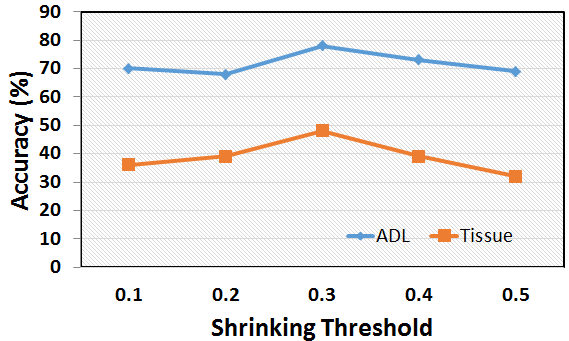
\includegraphics[scale=0.5]{Emp_up}
  \caption[Classification accuracy on validation set using the GKS method with different shrinking threshold values]{\fontsize{10}{12}\selectfont Classification accuracy on validation set using the GKS method with different shrinking threshold values}\label{ch3:fig:emp1}
\end{figure}
Moreover, the GKS method uses a shrinking threshold to eliminate similar points from the clusters. In this work, its value is empirically set to $0.3$ using its effect on classification accuracy on validation images. To visualize the same, Figure \ref{ch3:fig:emp1} shows the classification efficiency on the validation images of two considered datasets for different shrinking threshold values. It can be observed from the figure that the classification accuracy on ADL and Blue histology datasets are higher at the shrinking threshold $0.3$. The other parameter in the new GKS is the number of clusters for approximate k-means which is also set empirically to $1000$.
 

The performance of the GKS method is measured in terms of a number of selected keypoints and average computation time taken by the considered algorithms. Table \ref{ch3:tab:selectK} depicts the total number of extracted keypoints from SURF and selected keypoints by the proposed and the considered algorithms over two datasets. The percentage of the eliminated keypoints is also mentioned for each algorithm on the different datasets in parenthesis. Table \ref{ch3:tab:selectK} also depicts the average computational time taken by the different algorithms. From the table, it can be observed that the IB3 algorithm eliminates $85\%$ and $64\%$  keypoints from ADL and Blue histology datasets respectively. However, it consumes more computational cost as its complexity is $O(n^2log_2n)$ \cite{aha1991}. From Table \ref{ch3:tab:selectK}, it can be observed that IKS1 and IKS2 methods eliminate almost similar amount of keypoints ($41\%$ \& $44\%$) for Blue histology dataset. However, for ADL dataset, the reduction rate of IKS1 ($74\%$) is higher than IKS2.  As far as time complexities are a concern, both the methods take lesser time than IB3. However, the time complexity of IKS2 is $O(nlog_kn)$ which is better than IKS1 whose complexity is $O(n^2)$, where $k$ is the number of clusters. As compared to the algorithms mentioned above, the new GKS method shows the best reduction rate along with an efficient computational cost. The GKS method eliminates $95\%$ and $68\%$ keypoints from ADL and Blue histology datasets respectively. The time complexity of the GKS method is similar to IKS2 i.e., $O(nlog_kn)$. However, the GKS method uses approximate K-means and GRA which take lesser time than K-means and Euclidean distance similarity measure, used by IKS2 respectively. This difference can be visualized from the average time taken, as mentioned in Table \ref{ch3:tab:selectK}.


\begin{table}
\renewcommand{\arraystretch}{1.5}
\centering
\footnotesize
\caption[Number of selected keypoints returned by IB3, IKS1, IKS2, and GKS on considered datasets along with their average computational cost]{\fontsize{10}{12}\selectfont Number of selected keypoints returned by IB3, IKS1, IKS2, and GKS on considered datasets along with their average computational cost. The best results are in bold.}
\begin{tabular}{cll|cc}
    \hline
    
\textbf{Methods}    & \multicolumn{2}{c}{ \textbf{Number of keypoints}} &  \multicolumn{2}{|c}{\textbf{Average computational time (in hours)}}   \\
\cline{2-5}
&\textbf{ADL}&\textbf{Blue histology}&\textbf{ADL}&\textbf{Blue histology}\\
\hline
Without keypoints selection        &    4177920    &    158720    \\
IB3 &  626688 (85\%) & 57139 (64\%) &85.71 & 15\\ 
IKS1        &    1100000 (74\%)    &    65948 (59\%)  & 40& 7    \\
IKS2        &    2003000 (52\%) &    70312 (56\%)     & 8 &3.5\\    
GKS        &    \textbf{203000 (95\%)}     &\textbf{51000 (68\%)}    &  \textbf{4} &\textbf{1}    \\
\hline
\end{tabular}
\label{ch3:tab:selectK}
\end{table}


\subsection{Classification Results of GKS based BOF Method} \label{subsec:2}
In this section, the efficiency of GKS for keypoints selection is validated through the BOF method for classifying the histopathological images. To make the training set, $30$ images per category are selected and the remaining images in each category are added to the validation set.  The size of the codebook is empirically set to 500 for visual word generation. 
\begin{figure}[t]
\centering
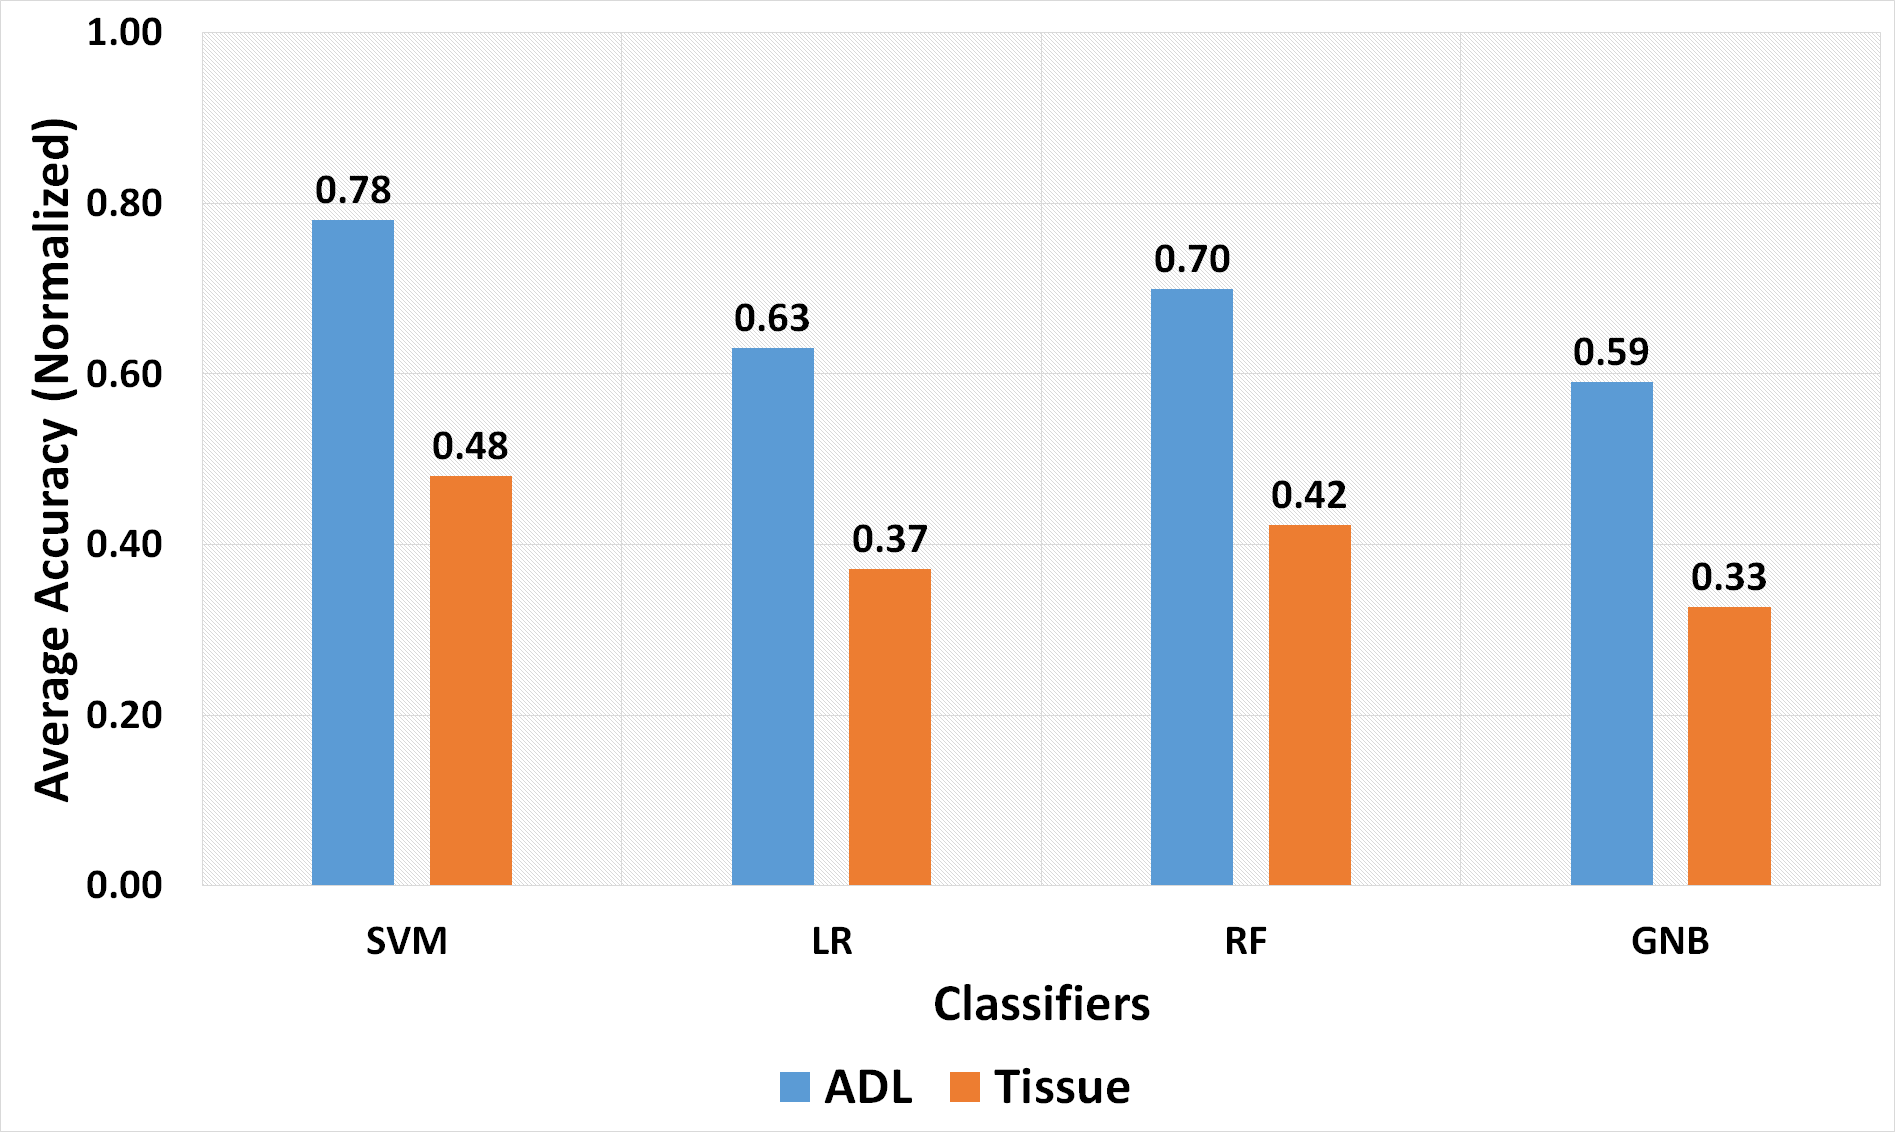
\includegraphics[scale=0.25]{SVM}
  \caption[Classification accuracy on validation set using the GKS method with different classifier on ADL and Blue histology datasets]{\fontsize{10}{12}\selectfont Classification accuracy on validation set using the GKS method with different classifier on ADL and Blue histology datasets}\label{ch3:fig:svm}
\end{figure}
Moreover,  the performance of GKS based BOF method is analyzed using four different classifiers, namely SVM, logistic regression (LR), random forest (RF), and Gaussian naive Bayes (GNN) classifiers. Figure \ref{ch3:fig:svm} shows the classification accuracy returned by the new method with different classifiers  on ADL and Blue histology datasets. From the figure, it can be visualized that the new method performs better when the SVM classifier is used. Hence, for further analysis, SVM is used as the classifier in the enhanced BOF method.

 For the classification of images using histograms, SVM classifier using error correcting codes (ECOC) \cite{ali2012} is used. ECOC is an efficient method to handle multi-class classification problems and is based on aggregating of the binary classifiers. Each considered binary classifier is independent. Efficient selection of kernel function is also desirable for better classification results. In this work, the $\chi^2$-kernel function is used instead of linear-kernel function due to its higher performance \cite{jiang2010}.  Moreover, tenfold cross-validation is applied to prevent the over-fitting problem. The random search is also used for hyperparameter tuning which uses uniformly distributed random values and finds the optimal combination in the parameter space.

\begin{figure}[h]
\centering
\subfigure[IB3]{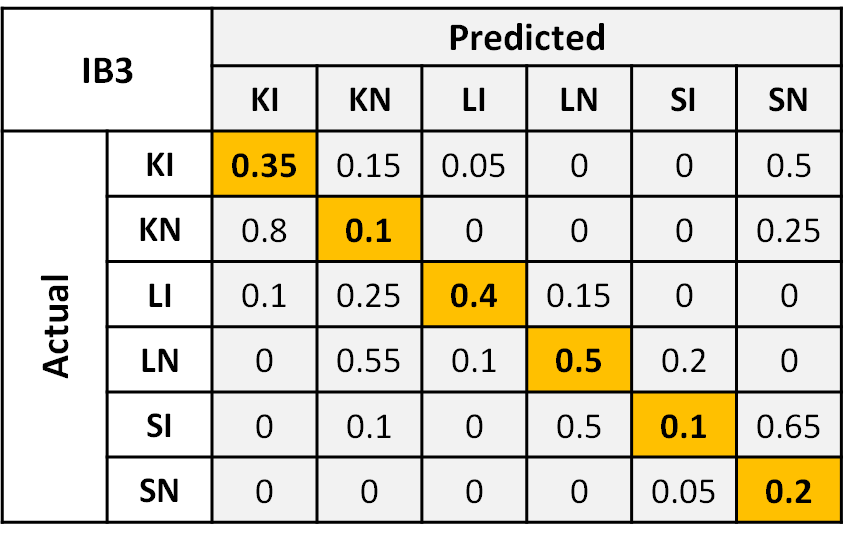
\includegraphics[width=0.33\linewidth]{CM-IB3-ADL}} ~
\subfigure[IKS1]{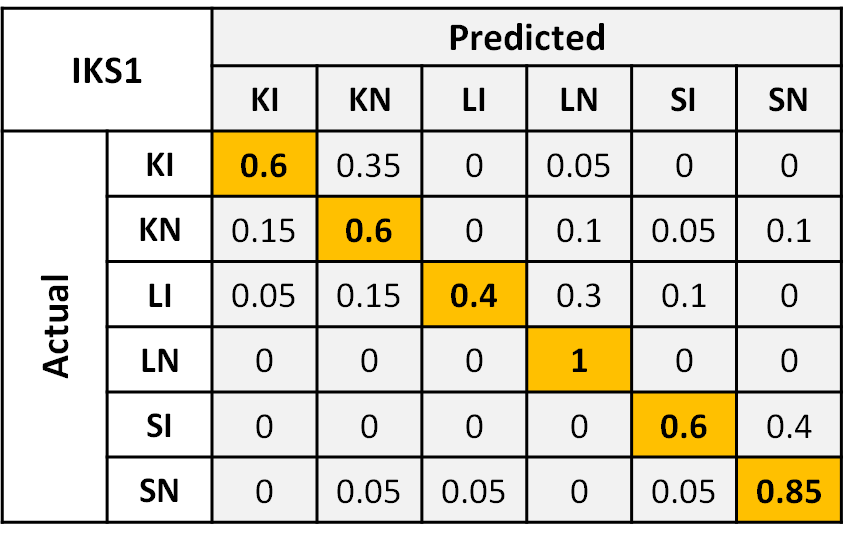
\includegraphics[width=0.33\linewidth]{CM-IKS1-ADL}}\\
\subfigure[IKS2]{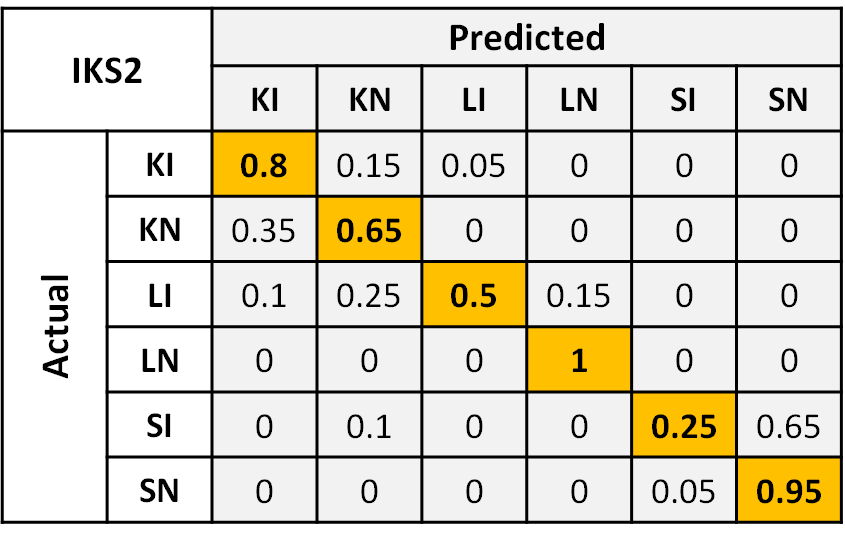
\includegraphics[width=0.33\linewidth]{CM-IKS2-ADL}}~
\subfigure[GKS]{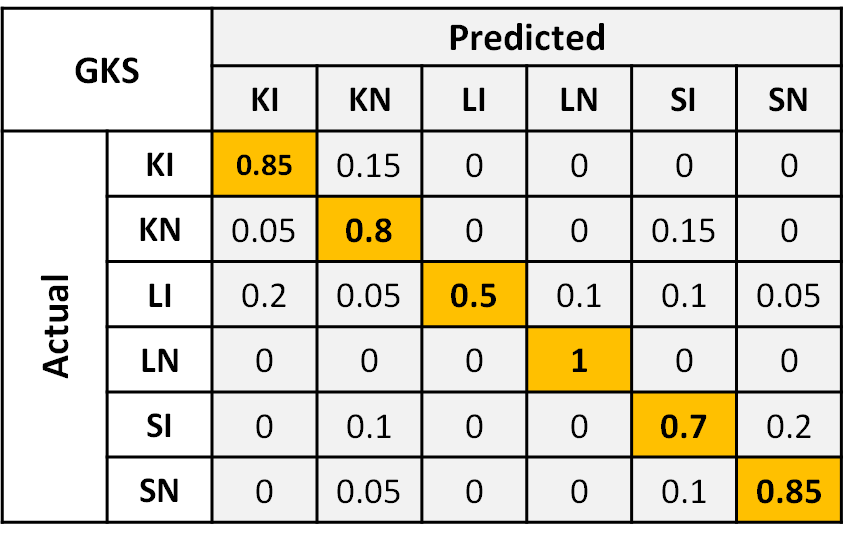
\includegraphics[width=0.33\linewidth]{CM-GKS-ADL}}
\caption[ The confusion matrices for the ADL dataset,  generated by IB3, IKS1, IKS2, and GKS based classification methods]{\fontsize{10}{12}\selectfont The confusion matrices for the ADL dataset,  generated by (a) IB3, (b) IKS1, (c) IKS2, and (d) GKS based classification methods. Here, KI: Kidney-Inflamed, KN: Kidney-Normal, LI: Lung-Inflamed, LN: Lung-Normal, SI: Spleen-Inflamed, and SN: Spleen-Normal.}
\label{ch3:fig:CMADL}
\end{figure}
\begin{figure}[h]
\centering
\subfigure[IB3]{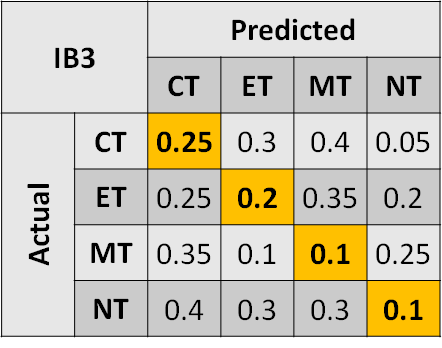
\includegraphics[height=1.5in, width=2.2in]{CM-IB3-Tissue}} ~~
\subfigure[IKS1]{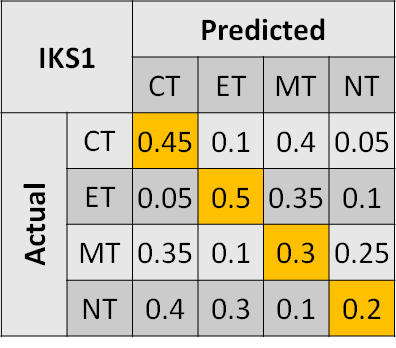
\includegraphics[height=1.5in, width=2.2in]{CM-IKS1-Tissue}}\\
\subfigure[IKS2]{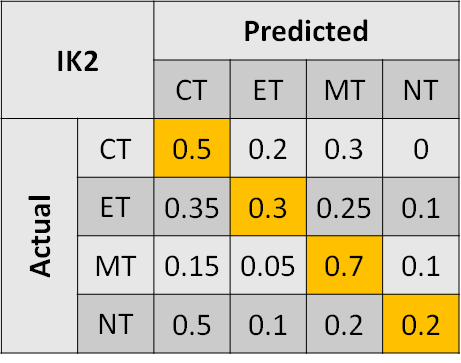
\includegraphics[height=1.5in, width=2.2in]{CM-IKS2-Tissue}}~~
\subfigure[GKS]{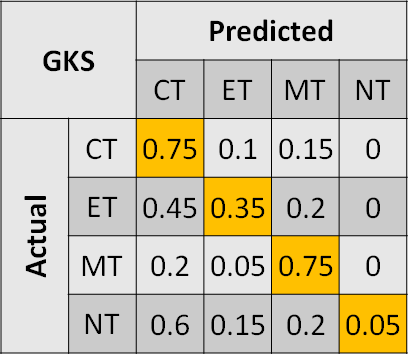
\includegraphics[height=1.5in, width=2.2in]{CM-GKS-Tissue}}
\caption[The confusion matrices for the Blue histology dataset, generated by IB3, IKS1, IKS2, and GKS based classification methods]{\fontsize{10}{12}\selectfont The confusion matrices for the Blue histology dataset, generated by (a) IB3, (b) IKS1, (c) IKS2, and (d) GKS based classification methods.}
\label{ch3:fig:CMTissue}
\end{figure}
Figure \ref{ch3:fig:CMADL} and \ref{ch3:fig:CMTissue} show the confusion matrices, generated by each considered method over ADL and Blue histology datasets respectively. The confusion matrices for ADL dataset show that IB3 based BOF method does not perform well on any of the classes, although it eliminates a significant amount of keypoints as shown in Table \ref{ch3:tab:selectK}. That's means, it does not select the prominent keypoints. The performance of both the IKS1 and  IKS2 is far better than IB3 for all the classes. However, IKS2 is slightly better than IKS1 for identifying kidney inflamed (KI) class and spleen normal (SN) class images. The performance of the new GKS based BOF method is tremendous in identifying the images of all the classes more accurately. It identifies all the lung-normal images from the ADL dataset while the worst performance is observed in the case of the lung-inflamed class which is also the best as compared to other methods.
Likewise, Figure \ref{ch3:fig:CMTissue} shows the confusion matrices for the Blue histology dataset, returned by IB3, IKS1, IKS2, and GKS based BOF methods. It can be seen from the figure that a classification accuracy of $75\%$ is returned by the GKS based BOF method for connective and muscle tissues which is better as compared to other methods. For epithelial tissue, IKS1 shows slightly better classification accuracy than the new method. For nervous tissue, IKS1 and IKS2 based methods outperform GKS and classify the images with equal accuracy. Similar to ADL dataset, IB3 does not perform well for the Blue histology dataset too. 

To analyze the results of confusion matrices quantitatively, recall, precision, F1-measure, specificity, and average accuracies are measured and depicted in Table \ref{ch3:tab:adl} and \ref{ch3:tab:tissue} for ADL and Blue histology datasets respectively.  
\begin{table}[t!]
\renewcommand{\arraystretch}{1.2}
    \centering
    \footnotesize
    \caption[Comparative analysis of the GKS based BOF method with other considered methods for ADL dataset in terms of various performance parameters]{\fontsize{10pt}{12pt}\selectfont Comparative analysis of the new GKS based BOF method with other considered methods for ADL dataset. The best results are in bold.    }
    \label{ch3:tab:adl}
    \begin{tabular}{|p{1.5in}|p{1.5in}|c|c|c|c|c|c|}
        \hline
        \textbf{Category}   &    \textbf{Parameters}    &    \textbf{IB3}    &    \textbf{IKS1}    &    \textbf{IKS2}    &    \textbf{GKS}    \\
     \hline
      Kidney - inflammation    &    Recall    &    33    &    60    &    80    &\textbf{    85    }\\
        &    Precision    &    28    &    75    &    64    &\textbf{    77    }\\
        &    F-measure    &    30    &    67    &    71    &\textbf{    81    }\\
        &   Specificity &   82  &   \textbf{96}  &   91  & 95\\
        \hline
        Kidney - normal    &    Recall    &    9    &    60    &    65    &\textbf{    80    }\\
        &    Precision    &    9    &    52    &    57    &\textbf{    70    }\\
        &    F-measure    &    9    &    56    &    60    &\textbf{    74    }\\
        &   Specificity &   79  &  89  &   90  & \textbf{93}\\
        \hline
        Lung - inflammation    &    Recall    &    44    &    40    &    50    &\textbf{    50    }\\
        &    Precision    &    73    &    89    &    91    &\textbf{    100    }\\
        &    F-measure    &    55    &    55    &    65    &\textbf{    67    }\\
        &   Specificity &   97  &  99  &   99  & \textbf{100}\\
        \hline
        Lung - normal    &    Recall    &    37    &    99    &    99    &\textbf{    100    }\\
        &    Precision    &    43    &    69    &    87    &\textbf{    91    }\\
        &    F-measure    &    40    &    82    &    93    &\textbf{    95    }\\
        &   Specificity &   86  &  91  &   97  & \textbf{98}\\
        \hline
        Spleen - inflammation    &    Recall    &    7    &    60    &    25    &\textbf{    70    }\\
        &    Precision    &    29    &    75    &    83    &\textbf{    67    }\\
        &    F-measure    &    12    &    67    &    38    &\textbf{    68    }\\
        &   Specificity &   95  &  96  &   \textbf{99}  & 93\\
        \hline
        Spleen - normal    &    Recall    &    80    &    85    &\textbf{    95    }&    85    \\
        &    Precision    &    13    &    63    &    59    &\textbf{    77    }\\
        &    F-measure    &    22    &    72    &    73    &\textbf{    81    }\\
        &   Specificity &   76  &  90  &   87  & \textbf{95}\\
        \hline
    & Average Accuracy ($\%$) &  27 & 68 & 69 & \textbf{78}\\
    \hline    
    \end{tabular}
\end{table}
\begin{table}
\renewcommand{\arraystretch}{1.2}
\centering
\footnotesize
    \caption[Comparative analysis of the new GKS based BOF method with other considered methods on blue histology tissue image dataset in terms of of various performance parameters]{\fontsize{10pt}{12pt}\selectfont Comparative analysis of the new GKS based BOF method with other considered methods on blue histology tissue image dataset. The best results are in bold.}
    \label{ch3:tab:tissue}
    \begin{tabular}{|p{1.5in}|p{1.5in}|c|c|c|c|c|c|}
\hline
\textbf{Category}   &    \textbf{Parameters}    &    \textbf{IB3}    &    \textbf{IKS1}    &    \textbf{IKS2}    &    \textbf{GKS}    \\
\hline
   &    Recall    &    13    &    30    &    70    &\textbf{    75    }\\
Muscle      &    Precision    &    9    &    26    &    48    &\textbf{    58    }\\
  Tissue  &    F-measure    &    10    &    28    &    57    &\textbf{    65    }\\
    &   Specificity &   66  &   72  &   75  & \textbf{    82    }\\
\hline
     &    Recall    &    25    &    45    &    50    &\textbf{    75    }\\
  Connective  &    Precision    &    20    &    36    &    33    &\textbf{    38    }\\
  Tissue  &    F-measure    &    22    &    40    &    40    &\textbf{    50    }\\
    &   Specificity &   66  &   \textbf{73}  &   67  &    58    \\
\hline
     &    Recall    &    20    &    34    &    30    &\textbf{    35    }\\
Epithelial    &    Precision    &    22    &    50    &    46    &\textbf{    54    }\\
  Tissue  &    F-measure    &    21    &    40    &    36    &\textbf{    42    }\\
    &   Specificity &   75  &   83  &   88  &\textbf{    90    }\\ 
\hline
     &    Recall    &    9    &    18    &\textbf{    20    }&    5    \\
Nervous    &    Precision    &    17    &    33    &    50    &\textbf{    100    }\\
 Tissue   &    F-measure    &    12    &    25    &\textbf{    29    }&    10    \\
    &   Specificity &   82  &   87  & 93 & \textbf{100}\\
\hline
& Average Accuracy ($\%$) &  17 & 36 & 43 & \textbf{48}\\
\hline
\end{tabular}
\end{table}
From Table \ref{ch3:tab:adl}, it can be stated that GKS outperforms the other methods for almost all the parameters. Furthermore, the average classification accuracy of GKS on ADL dataset is $78\%$ which is higher than other considered state-of-the-art methods, i.e., IB3, IKS1, and IKS2 which give $27\%$, $68\%$, and $69\%$ accuracy respectively. Likewise, the new method also shows the best performance for all the tissue classes of Blue histology dataset with F1-measures equals to $65\%$, $50\%$, and $42\%$  for muscle, epithelial, and connective respectively except nervous tissue where IKS2 shows better results. Moreover, the overall accuracy of the new method for the Blue histology dataset is $48\%$ while IB3, IKS1, and IKS2 return $17\%$, $36\%$, and $43\%$ accuracy respectively. However, the accuracy on the Blue histology dataset is not up to the mark due to the lots of staining variations available in the images of the Blue histology dataset as depicted in Table \ref{ch3:tab:tissued}. Especially, in the nervous tissue, LFC staining images are very much different from nervous tissue images. Therefore, its performance is degraded in all the methods.

From the results, it can be stated that the classification accuracy of the GKS based BOF method is better than the other considered methods. The baseline algorithm (IB3) gives poor performance in all scenarios as it filters out a large number of keypoints including the relevant ones. This reduces the size but also degrades the classification performance. IKS2 performs better than IKS1 as it starts with multiple reference points together and applies the reduction phase cluster-wise to reduce the overall training set. Therefore, IKS2 is fast and efficient than IKS1.  In the new GKS method, the use of Grey relational analysis based similarity measure and approximate K-means make it faster and efficient. As the number of keypoints is reduced, the number of visual words is also reduced in the GKS based BOF method.
\begin{figure}[h]
\centering
\subfigure[ADL dataset]{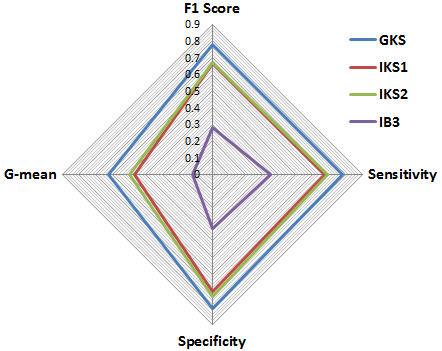
\includegraphics[width=0.45\linewidth]{radar_ADL}}
\subfigure[Blue histology dataset]{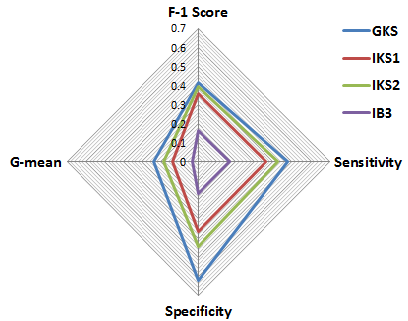
\includegraphics[width=0.45\linewidth]{radar_tissue}}
 \caption[Radar charts for average results obtained for SVM classifier on ADL dataset and Blue histology image dataset by considering F-1 score, sensitivity, specificity, and G-mean]{\fontsize{10pt}{12pt}\selectfont Radar charts for average results obtained for SVM classifier on a) ADL dataset and b) Blue histology image dataset by considering F-1 score, sensitivity, specificity, and G-mean}
\label{ch3:fig:rc}
\end{figure}

However, accuracies of the classifiers may not be the appropriate performance metric if the number of inflamed images is larger than the number of normal images. For example, if there are $1000$ histopathological images in which $995$ images are normal and $5$ images are inflamed. If the proposed method classifies all images as inflamed, then the accuracy would be $99.5\%$. However, the method miss-classify  all the normal cases. To mitigate this, G-mean ($\sqrt{TP*TN}$) is considered as the performance metric which includes true positives (TP) and true negatives (TN) in a product. Furthermore, the performance of IB3, IKS1, IKS2, and GKS methods are also analyzed using radar charts which are shown in Figure \ref{ch3:fig:rc} that depict four evaluation criteria, namely F1 score, sensitivity, specificity, and G-mean which resulting in four-sided shape. The method with a maximum area and symmetrical shape perform better than others. From the figure, it can be observed that the GKS based BOF method achieves better results among all the other methods in four considered measures. Therefore, it can be stated that the new keypoints selection in the BOF method outperforms the other keypoints selection methods and may be applied for histopathological image classification.

\subsection{Comparative Analysis of GKS based BOF with State-of-the-Art Methods }\label{ch3:subsec:3}

The performance of the GKS based BOF method is also compared with the three state-of-the-art methods for ADL histopathological image dataset, namely WND-CHARM \cite{shamir2008}, SRC \cite{wright2009}, and SHIRC \cite{srinivas2014} in terms of recall, specificity, precision, false negative rate (FNR), average accuracy, and F1-score. Shamir et al. \cite{shamir2008} introduced a method for the analysis of biological images in which image content features are detected from the raw images and selected informative feature descriptors are used to train the classifier. In the sparse representation-based classification (SRC) method \cite{wright2009}, RGB images are represented by a single luminance channel and this representation is used to train the classifier. Moreover, this work is further extended to three color channels and known as a multi-channel simultaneous sparsity model (SHIRC) \cite{srinivas2014}. This method is also analyzed and validated on ADL histopathological images. Table \ref{ch3:tab:adlp} shows the results of each considered method on the various performance parameters, namely recall, specificity, precision, false negative rate (FNR), and F1-score to identify the inflamed images of each organ in ADL dataset.
\begin{table}
\centering
\footnotesize
\caption[Classification performance of GKS based BOF method with other methods]{\fontsize{10pt}{12pt}\selectfont Classification performance of GKS based BOF method with other state-of-the-art methods}
    \label{ch3:tab:adlp}
\renewcommand{\arraystretch}{1.3} 
\begin{tabular}{|c|l|c|c|c|c|c|c|}
\hline
\textbf{    Organ     }&\textbf{    Algorithms    }&\textbf{    Recall    }&\textbf{    Specificity    }&\textbf{    Precision    }&\textbf{    FNR    }&\textbf{    F1-score    }&\textbf{    Avg. Accuracy ($\%$)}\\
        \hline


        &    WND-CHARM    &    0.690&0.720& 0.710 & 0.280    &    0.700    &    71.0    \\
    &    SRC    &    0.875    &    0.750    &    0.778    &    0.250   &    0.825    & 81.3       \\
Kidney    &    SHIRC    &    0.825 & 0.833 &   0.832   & 0.167    &    0.828    & 82.9        \\
    &    BOF    &    0.870    &    0.650    &    0.731    &    0.350   &    0.826    &  80.0      \\
    &    GKS    &\textbf{    0.950    }&\textbf{    0.890    }&\textbf{    0.888    }&\textbf{    0.110    }&\textbf{     0.879   }&\textbf{    88.0    }\\
    \hline
    &    WND-CHARM &  0.725  & 0.626 &  0.705    &    0.374    &   0.791     &       75.7 \\
    &    SRC    &   0.880    &    0.765    & 0.750    &    0.235    &    0.737    &  74.5      \\
Lung    & SHIRC &  0.750& 0.850    &    0.833    &    0.150    &   0.791    &    80.0     \\
    &    BOF    & 0.730    &    0.750    &    0.745    &    0.250    &   0.737     &    74.0    \\
    &    GKS    & \textbf{ 0.888}    &\textbf{    0.860    }&\textbf{    0.863    }&\textbf{    0.140    }&\textbf{    0.871    }&\textbf{ 87.0       }\\
    \hline
    &    WND-CHARM    &    0.512    &    0.873    &    0.800    &    0.128    &    0.640    &     69.2   \\
    &    SRC    &    0.708    &    0.792    &    0.773    &    0.208    &   0.740     &   75.0     \\
Spleen    &    SHIRC    &    0.650    &    0.883    &    0.848    &    \textbf{   0.117  }  &     0.742    &   76.7    \\
    &    BOF    &    0.880    &    0.530    &    0.652    &    0.470    &      0.749   &  70.5     \\
    &    GKS    &\textbf{    0.750    }&\textbf{    0.880    }&\textbf{    0.862    }& 0.120    &\textbf{   0.804    }&\textbf{   81.5      }\\
\hline
\end{tabular}
\end{table}
Recall and specificity are the two key statistics to validate the performance of classification in medical diagnosis. Recall is the probability to identify diseased images correctly, while specificity returns the probability of identifying the healthy images correctly. In histopathological image analysis, it is always important to identify inflamed images with higher accuracy. From Table \ref{ch3:tab:adlp}, it can be noticed that the new GKS method has high recall values of $95\%$, $88.8\%$, and $75\%$ for Kidney, Lung, and Spleen organs respectively. Moreover, the true negative rates returned by the GKS method are 89\%, 86\%, and 88\% for Kidney, Lung, and Spleen organs respectively. Hence, it can be stated that the GKS method also identifies healthy images more accurately as compared to the other considered methods.  Further, the GKS based BOF method also attains high average accuracy, precision, and F-1 score. The results have also been analyzed on the FNR which can be defined as the rate of identifying inflamed images as healthy images. It is very dangerous in medical diagnosis and it should be minimized. The GKS method has the lowest FNR of 11\% and 14\% on Kidney and Lung organ images respectively. However, for Spleen organ images SHIRC outperforms the GKS method in terms of FNR. 

\section{Summary}\label{sec:con}
In this chapter, a new GKS method of keypoints selection has been presented which improves the efficiency of the bag-of-features method. The method uses Grey relational analysis and approximate K-means for the elimination of irrelevant and similar keypoints.  Furthermore, the new keypoint selection method has been incorporated in the BOF method to reduce its computational complexity. Moreover, the support vector machine is used to train and classify the images into respective categories. The GKS based BOF method is tested on two complex histopathological image datasets. The simulation results and classification accuracy show the efficacy of the new method on the other considered methods. 

The next chapter introduces an optimal codebook construction method to be used in the BOF for histopathological image classification.


